\documentclass[13pt]{report}
\usepackage[utf8]{inputenc}
\usepackage{graphicx}
\usepackage[margin= 1in]{geometry}
\usepackage{titlesec}
\usepackage{url}
\usepackage{float}
\usepackage{mathtools}
\usepackage{amsmath}
\usepackage{multirow}

\usepackage{tikz}
\usetikzlibrary{shapes.geometric, arrows}
\tikzstyle{startstop} = [rectangle, rounded corners, minimum width=3cm, minimum height=1cm,text centered, draw=black, fill=white]

\tikzstyle{io} = [trapezium, trapezium left angle=70, trapezium right angle=110, minimum width=3cm, minimum height=1cm, text centered, draw=black, fill=white]

\tikzstyle{process} = [rectangle, minimum width=3cm, minimum height=1cm, text centered, draw=black, fill=white]

\tikzstyle{decision} = [diamond, minimum width=3cm, minimum height=1cm, text centered, draw=black, fill=white]

\tikzstyle{arrow} = [thick,->,>=stealth]

\setlength{\parskip}{1em}
\setlength{\parindent}{0em}
\graphicspath{{images/}}
\titleformat*{\section}{\LARGE\bfseries}
\titleformat*{\subsection}{\Large\bfseries}
\titleformat*{\subsubsection}{\large\bfseries}
\titleformat*{\paragraph}{\large\bfseries}
\titleformat*{\subparagraph}{\large\bfseries}



% Title Page
\title{
	{Financial Forecasting: Changepoint Detection In Financial Time Series Using LAGRAMGE}\\
	{University of York}\\
	{
\includegraphics[scale=0.5]{uoycrest.jpg}}
	}	
\author{Aisha Animashaun}


\begin{document}

\maketitle
\pagenumbering{roman}
\tableofcontents
\listoffigures
\listoftables
\chapter*{Acknowledgements}
\begin{abstract}
\end{abstract}
\pagenumbering{arabic}
\chapter{Introduction}
\chapter{Literature Review}
A Financial market is defined as a highly competitive market dealing in financial instruments; these financial instruments are readily negotiable claims such as securities, futures contracts, and options~\cite{houthakker1996economics}. The purpose of a financial market is to facilitate: the establishment of a price for global trade, transfer of liquidity and risk, and raising of capital~\cite{investopediafinancialmarketsdef}. Investors participate in a financial market to achieve different objectives; ranging from seeking a regular income, to the pursuit of a significant appreciation of their capital. Regardless of an investor's objective,being able to closely predict the behaviour of prices is necessary for their achievement.\par

This section of this paper discusses...

\section{The Efficient Market Hypothesis}
Prices in financial markets are typically reactive to all events, both real and those imagined by the collective intelligence of the markets~\cite{cootner1964random},therefore, they are difficult to predict accurately; this forms the basis for the Efficient Market Hypothesis (EMH). Founded by Eugene F. Fama in the 1960s, the EMH asserts that the stock market is informationally efficient, that is, all available information at a particular time is fully reflected in current prices; implying the lack of opportunity to predicatbly or consistently earn higher than average returns by investing on the basis of information already available to other market participants~\cite{houthakker1996economics}~\cite{clarke2001efficient}. \par

The EMH has three main variants: the weak form which considers only past prices; the semi-strong form which also considers information made available to the public; and the strong form, which considers non-public information in addition to the information considered by the other variants \cite{houthakker1996economics}. If the weak form holds, prices will exhibit a simple form of the martingale model, the random walk~\cite{bailey2005economics}; this idea is based on the consideration that if stock prices are responding to a random sequence of events or information, then they will consequently follow a random walk\cite{houthakker1996economics}. The random walk of asset prices can be written as \[E[p_{t+1}|\Omega_{t}]=p_{t}\] where \(p_{t}\) denotes the price of an asset at time \(t\); and \(\Omega_{t}\) represents the set of information available at time \(t\), and it must at least include all the past prices of the asset, that is \(\Omega_{t}= \left\{p_{t}, p_{t-1},...\right\}\). The random walk model suggests a price series where all subsequent changes in price represent random departures from previous prices~\cite {pricesmalkiel2003efficient}. Statistically, the random walk model indicates independence between price changes, that is, the probability distribution for the price change during time $t$ is independent of the previous price changes; therefore, knowledge of previous price changes gives no insight when assessing the probability distribution for the price change at time $t$~\cite{fama1965behavior}.\par

If prices follow a a random walk, then the activity of investing in a financial market can be likened to gambling, where the ownership of an asset is perceived as participation in a fair game, where the expected gain or loss is zero~\cite{bailey2005economics}. The formula for this concept is derived from that of the random walk by subtracting $p_{t}$ from $p_{t+1}$ and $p_{t-1}$ from $p_{t}$ \[E[p_{t+1}-p_{t}|\Omega_{t}]=0\] 

This model of a fair game is convenient for empirically testing the random walk hypothesis. Tests developed for the random walk hypothesis are often based on sample autocorrelation coefficients, using a time series of data on an asset, or a portfolio of assets. If the behaviour of the price or prices being studied follow a random walk, then the autocorrelation coefficients should equal zero~\cite{bailey2005economics}. 

Researchers have conducted various studies to decide whether or not stock prices follow a random walk; this is evident in the ample amount of literature available for this topic, and as with many prominent research topics, the statistical results vary. Some research reject the random walk hypothesis by providing evidence that the autocorrelation coefficients for a time series sample is non-zero; hence suggesting that prices are predictable. Using a simple specification test based on variance estimators and 1216 weekly observations over a twenty-three year period, Lo and Mackinlay compute the weekly first-order autocorrelation coefficient of the equal-weighted CRSP index to be thirty percent,thus rejecting the random walk hypothesis~\cite{lo1988stock}. Worthington and Higgs also reject the random walk behaviour for Latin American stock markets by employing tests for autocorrelation coefficients, and using daily data for up to a fifteen year period~\cite{worthington2003empirical}. Evidence of mean reversion, where assets with low average returns experience a rise in return and conversely for assets with high average returns, also exists for over long periods of time, such as several years or decades; suggesting the predictability of prices~\cite{bailey2005economics}. Using the national stock index data of eighteen countries over a period of three years, and employing methods that exploit cross-sectional variation as a test for mean reversion, Balvers et al. reject the absence of mean reversion at the 5 or 1 percent
significance level, thereby reporting strong evidence of mean reversion in relative stock index prices. From their research results, they infer that parametric contrarian investment strategies that fully exploit mean reversion across national indexes outperform a number of other investment strategies~\cite{balvers2000mean}.

On the other hand, researchers who believe that prices follow a random walk argue that, although there are apparent cycles in the times series of a stock price, randomly generated series also display cycles. In addition to research where the statistical tests employed accept the null hypothesis, the random walk is also supported by an argument based on the fair coin, that is, if one tosses a fair coin many times, a flow of heads will be followed by a flow of tails; therefore cycles observed in the behaviour of stock prices occur by chance and their occurence is unpredictable~\cite{houthakker1996economics}. In their research to examine the market efficiency of twenty European equity markets, of which sixteen are regarded as developed and the others as emerging, Worthington and Higgs employ a combination of autocorrelation coefficient and runs tests, an Augmented Dickey-Fuller
(ADF) test, a Phillips-Perron(PP) test, and a Multiple Variance Ratio (MVR) test; they report that Hungary, Germany, Ireland, Portugal, Sweden, and the United Kingdom are characterised by a random walk~\cite{worthington2004random}. Borges also gives evidence supporting the weak-form market efficiency, that is, the random walk. Borges employs an autocorrelation coefficient test, a runs test, an augumented Dickey-Fuller test, and the multiple variance ratio test proposed by Lo and MacKinlay to test the hypothesis, using daily and monthly data for the stock market indexes of France, Germany, United Kingdom, Greece, Portugal and Spain, from a period of fourteen years. They report that monthly prices and returns follow a random walk in all the countries examined~\cite{borges2010efficient}. For the reader's interest, Shamshir and Mustafa provide a more exhaustive account of existing empirical evidence regarding the random walk in stock markets~\cite{shamshirefficiency}.\par

A major limitation to tests of the EMH is the absence of a precise specification of what constitutes an "efficient" price response to information; this limitation brings about the bad model problem~\cite{ball2009global}. Any test for market efficiency must assume an equilibrium model that defines normal security returns; if a test rejects efficiency, it can be as a result of the market truly being inefficient, or as a result of an incorrect assumption of the equilibrium model~\cite{campbell1997econometrics}.This joint hypothesis problem means that market efficiency as such can never be rejected~\cite{campbell1997econometrics}. Further limitations to tests of the EMH are enlisted in~\cite{campbell1997econometrics}; the overarching point is that the real world is complex, therefore many of the models used to test the EMH by researchers could be too simple to arrive at a conclusion on the efficiency of markets.\par

Campbell et al. maintain that the concept of perfect market efficiency is an unrealistic benchmark unlikely to hold in theory and practice. They advocate that contrary to the EMH which assumes information processing to be costless, abnormal returns exist in the market if there are costs of gathering and processing information, and such abnormal returns are necessary  for compensating investors~\cite{campbell1997econometrics}.\par

Relative efficiency has been proposed as a more useful concept than the hard-line approach taken by most traditional market-efficiency literature~\cite{campbell1997econometrics}, however, the literature available for this concept is minimal in comparison to the EMH. The notion of relative efficiency is based on whether one market is more or less efficient than another according to a specific criteria or efficiency model~\cite{bailey2005economics}. Comparisons for relative efficiency might be between different market locations, different parts of the same market, or the same market at different points in time. In order to make inferences about relative efficiency, tailored methods must be employed for ranking various degrees of inefficiency.In the paper, 'Ranking efficiency for emerging markets', Cajueiro amd Tabak test for long range dependence and efficiency in stock indices for thirteen markets, of which eleven are categorised as emerging, and the remainder as developed.To investigate the relative efficiency of these equity markets, they employ a "rolling sample" approach and calculate median Hurst exponents, $R/S$ and modified $R/S$ statistics. They report results suggesting that most Latin American equity markets show greater efficiency than those of Asian equity markets; they also report that developed markets rank first in terms of efficiency~\cite{efficiencycajueiro2004ranking}. Lim also presents a paper based on ranking market efficiency for stock markets, but from a non-linear perspective. Also using a rolling sample approach and a similar data sample to~\cite{efficiencycajueiro2004ranking} , he demonstrates that the non-linear dependence in stock returns is seemingly localised in time, suggesting that market efficiency evolves over time. As the rolling sample approach is able to detect periods of efficiency and inefficiency, the relative efficiency of stock markets are easily assessed by comparing the total time windows these markets exhibit significant non-linear serial dependence; he reports results suggesting that the United States market is most efficient while Argentine is the least~\cite{efficientlim2007ranking}. The results of studying the relative efficiency of markets can be employed to create efficient market investment strategies across markets. 

\section{Forecasting Financial Markets}
Regardless of the abundant research reporting results that suggest market efficiency, investing in the financial markets is still viewed as a lucrative option for many individuals and companies. The primary motive of  investors is to buy shares at a relatively low price and sell them at a higher price; this price change and dividends constitute the expected returns from investing in financial markets~\cite{kevin2015security}. Therefore, investors are customarily interested in the future value of these expected returns, and endeavour to carry out rational investment activity by attempting to forecast the behaviour of an asset. Financial market forecasting is an attempt to determine the future value of a financial instrument; this value can only be estimated and not predicted with certainty. The fascination and challenges of this problem is emphasised by the number of prominent academicians that have applied their skills to forecasting financial instruments. Moreover, successful participants in financial markets often rationalise their survival by their ability to recognise the behaviour of a promising asset, in other words, their ability to predict patterns in asset prices~\cite{bailey2005economics}.\par 

This section aims to present various approaches to financial market forecasting. These include: security analysis, which is generally split into fundamental and technical analysis; and equation discovery methods.

\subsection{Fundamental Analysis}
Fundamental analysis is based on the premise that the price of an asset is determined by a number of fundamental factors relating to the economy, industry and company~\cite{kevin2015security}. Each asset in a financial market is assumed to have an intrinsic or fundamental value, that is, its economic worth based on its present and future earning capacity. The purpose of fundamental analysis is to assess the intrinsic value of a financial asset, by evaluating its present and future earning capacity~\cite{kevin2015security}. The aim of deriving the intrinsic value is to provide an investor a standard with which to compare the asset's prevailing market price, and arrive at an investment decision. If during comparison, the prevailing market price is observed as being lower than the intrinsic value, then the asset is viewed as under-priced and a good investment opportunity for participants~\cite{kevin2015security}. However, if the prevailing market price is higher than the intrinsic value, the asset is categorised as being overpriced, and the investor would probably decide to sell off such an asset, or resist from investing in the asset~\cite{kevin2015security}. 

Although the line between a rumour and accurate information is very thin, and using tips might truly help an investor outperform the market, fundamental analysis insists that investors must not trade based on tips and rumours. Fundamentalists are expected to consistently employ the Economy-Industry-Company (EIC) framework when making trading decisions. The EIC is an analytical framework that affirms that detailed analyses of the information about the company, the industry to which the company belongs, and the economy constitute the main activities in the fundamental approach to security analysis~\cite{kevin2015security}.\par

Fundamental analysis is primarily criticised by two main groups: advocates of the EMH and technical analysts. According to Fama, a significant EMH proponent, fundamental analysis is only useful when an investor is trading in an inefficient market, because in efficient markets, asset prices will represent good estimates of intrinsic or fundamental values at any point in time~\cite{fama1995random}. Technical analysts also provide a similar criticism, they argue that by the time accurate and reliable information is obtained, it is woefully out of date; therefore, the fundamental factors considered by fundamentalists have no influence on current pricing trends. The argument proposed by technical analysts is based on the notion that, it is the timing of decisions that determines if an investor succeeds or fails in the financial markets~\cite{marketthomsett2006getting}.

The most famous and successful investor in the world, Warren Buffett, is a fundamental analyst who as part of his portfolio, trades in markets deemed efficient; thus rendering the arguments against fundamental analysis questionable. Furthermore, in their studies of the Japanese equity market, Chan et al.~\cite{chan1993can} and Andreas et al.~\cite{charitou2000value} report results that suggest the efficiency of fundamental analysis.

 

\subsection{Technical Analysis}
Technical analysis is traditionally defined as the forecasting of future price trends by using charts to study market action~\cite{murphy1999technical}. It is primarily based on the recognition of chart patterns, and is otherwise known as charting. The rationale for technical analysis is based on three premises. The first premise is that market action discounts everything; this is based on the assumption that any factor, whether fundamental, political, psychological or otherwise, that could possibly affect the price of an asset is already reflected in the asset's price~\cite{murphy1999technical}. The second and third premises respectively state that prices move in trends, and history repeats itself. Statistically, in direct contrast to the EMH, technical analysts assume that the successive price changes of a financial asset are dependent.\par

Various types of charts and market indicators are employed in technical analysis.The most widely used kind of chart is the daily bar chart which shows the open, high, low and closing prices for each day. Other types include the line charts, point and figure charts, and candlesticks. The objective of a technical analyst observing a chart is to identify certain types of patterns in the plotted behaviour of an asset's price. Types of patterns that are usually of interest to an analyst include but are not limited to 'Head and Shoulders', 'Cup and Handle', 'Triple Tops and Bottoms', 'Gaps', and 'Wedge'. Market indicators such as the Moving Average Convergence Divergence(MACD) which is used to measure momentum, and the Aroon Oscillator which is used to predict trend reversal; are just a few of the indicators used by technical analysts.\par

Traditional technical analysis as characterised by the analysis of charts to detect patterns is highly subjective, therefore, the recognition of geometric shapes in price charts is often in the eyes of the beholder~\cite{lo2000foundations}. According to Buffett, technical analysis does not work since the flipping of a chart supposedly does not give a different interpretation. Fama's argument against the effectiveness of technical analysis is that, with the strong support for the random walk model provided by empirical evidence, the work of a chartist is similar to that of an astrologer, hence it has no real value in the analysis of stock prices; he  challenges the chartist to present evidence that his techniques can consistently be used to make a better than chance predictions of the behaviour of an asset's price~\cite{fama1995random}. Another famous proponent of the EMH, Burton Malkeil, concludes that, "[u]nder scientific scrutiny, chart-reading must share a pedestal with alchemy." ~\cite{lo2000foundations, malkiel1999random} The line between investors that apply fundamental analysis, and those that use technical analysis to decide their investment activity is not rigid; there exists traders that believe fundamental analysis and technical analysis complement each other, and employ them together. Their reason for this is that it is illogical to attempt to forecast asset prices by observing a chart of past prices, without also considering financial statements or the surrounding economic conditions, and vice versa.\par


In the light of the scrutiny given to the attempt to forecast asset prices using just charting, pure chartists are increasingly rare in the financial markets, and technical analysis has evolved over the years to employ advanced quantitative methods to this challenge~\cite{methodslo2011evolution}. An  advantage of the evolution of technical analysis is that, the resulting methods are systematic and can be automated using computer programs. A further advantage is that the recognition of patterns can be rationalised using mathematical proofs or statistical tests. The basic assumption of technical analysis persists in the objective of the developed quantitative methods, which is to develop mathematical models that can be used to predict the future behaviour of an asset's price based on the previous prices. The field of economics dedicated to such quantitative research is econometrics, and these methods are centred on time series analysis. 

\subsection{Time Series Analysis: Econometric Models}
Time series analysis is a key concept in Econometrics. Econometrics is defined as the social science where tools of economic theory, mathematics and statistical inference are applied to the analysis of economic phenomena; the aim is to give a numerical estimate of the relationship between variables~\cite{gujarati1999essentials}. Time series analysis consists of methods for analysing time series data in order to identify the underlying process or model generating the sequence of observation. Identification and forecasting are the two main goals of time series analysis. The focus of this section is to present some of the key notions and methods in Time series analysis.\par

\subsubsection{The Stylised Facts of Financial Time Series}

\subsubsection{Stationarity, Ergodicity and White Noise}
The aim of this section is to present the three building blocks of time series models: stationarity, ergodicity and white noise.\par

The major properties of the underlying process for a time series can be described in terms of just its means and covariances; but these quantities are difficult to estimate with precision for an economic process~\cite{processgranger2014forecasting}. For example, when analysing the time series for the price of an asset, it is only possible to observe one realisation of the underlying process, that is, it is impossible to observe the various probable patterns that could arise for a particular starting point of an asset's price~\cite{processgranger2014forecasting}. In order to overcome this limitation, some restrictive but usable assumptions about the way means and covariances change over time are adopted by time series analysts~\cite{processgranger2014forecasting}. Stationarity is one of such assumptions.\par

A process $X_{t}$ is said to be stationary if the potential distribution of its realisations at time $t$ has a mean and variance that is independent of time; and if the covariance between its values at any two points in time depends only on the distance between them, and not on time~\cite{dougherty2007introduction,processgranger2014forecasting}. It is important to clarify that under the assumption of stationarity, although  $X_{t}$ itself changes over time, the potential distribution of its realisations at any time $t$ does not change~\cite{dougherty2007introduction}. Hence, the focus is on the distribution of a cross-section of realisations of $X_{t}$, and not on its ordinary distribution~\cite{dougherty2007introduction}. Essentially, assuming an underlying process is stationary is equivalent to assuming that the underlying process of a time series is time-invariant~\cite{processgranger2014forecasting}. 

A further assumption made by time series analysts is ergodicity. A process is ergodic if the values at any two points that are sufficiently far apart in time are independent, in other words, uncorrelated~\cite{processgranger2014forecasting}. 
This is so that new and useful information is continually added to the average when averaging the series through time; thus, the resulting time average is an unbiased and consistent estimate of the population mean~\cite{processgranger2014forecasting}. This is the same for the covariance.Therefore, given the assumption of stationarity and ergodicity, analysts can form good estimates of the means and covariance of a process by averaging through time, rather than being forced to depend on the ensemble averages across realisations.

White noise is a process denoted as $\varepsilon_{t}$, it is defined as an independent and identically distributed random variable with zero mean. The mean, variance and covariance of a white noise are time invariant, therefore it is a stationary~\cite{processsheppard2013financial}. Models developed by time series analysts are characterised by a particular structure: the dependent variable or process that is observed often depends on specific independent or explanatory variables, and white noise.

In the following sections, three widely used models in the financial industry are presented.

\subsubsection{Mixed Autoregressive Moving Average Models}
Mixed autoregressive moving average models are denoted as $ARMA(p,q)$ and consist of two terms from two different processes: an autoregressive process and a moving average process ~\cite{parametershamilton1994time}. Autoregressive processes denoted $X_{t}\sim AR(p)$ are useful when describing situations where the current value of a time series is dependent on its previous values plus a random shock~\cite{wei1994time}. The general form of an AR model with order $p$ is \[X_{t}=\sum_{j=1}^{p}a_{j}X_{t-j}+\varepsilon_{t}\]\par

Moving average processes denoted $X_{t}\sim MA(q)$  are useful for describing situations where events produce an immediate effect that only lasts for short periods of time~\cite{wei1994time}. The general form of an MA model with order $q$ is \[X_{t}=\sum_{j=0}^{q}b_{j}\varepsilon_{t-j}, b_{0}=1\]\par

A stationary process or model can be expressed using just a moving average form, or an autoregressive form. However, the problem with using just one of these forms to represent a process is that the resulting model may contain too many parameters; this is because when used alone, they often produce a high order model for good approximation~\cite{wei1994time}. The problem with having too many parameters is similar to that highlighted by Occam's razor, the efficiency of the model is reduced when used for forecasting. Therefore, when building a model with the aim of forecasting, it may be necessary to include both autoregressive and moving average terms in the model to reduce the number of parameters, hence the $ARMA(p,q)$ process. The general form of an ARMA model with a pth order autoregressive process and a qth order moving average process is \[X_{t}=\sum_{j=1}^{p}a_{j}X_{t-j}+\varepsilon_{t}+ \sum_{j=0}^{q}b_{j}\varepsilon_{t-j}, b_{0}=1\] if $X_{t}$ is generated in this fashion, it is called a mixed ARMA process and denoted $X_{t}\sim ARMA(q)$. As a finite moving average process is always stationary, the restrictive assumption of stationarity in these types of models depends entirely on the autoregressive parameters~\cite{parametershamilton1994time}.\par

ARMA-type models are one of the simple and practical models in financial time series analysis that can predict the future value of an asset with relatively high accuracy~\cite{zhang2013research}. Due to the notion that the changing trend of Consumer Price Index (CPI) affects the degree of inflation to an extent, Zhang et al. conduct a study to find out the accuracy of using the ARMA process to model consumer price index. They use China's monthly CPI data from January 1995 to May 2008 to fit an ARMA(1,1) model, then test the accuracy of the model by making out-of-sample forecasts for the monthly CPI values from April to September 2008. They measure the relative error between the true value and predicted value for each forecasting month, and report all errors to be below one percent, thus concluding that the ARMA model is valid and has a relatively high forecasting accuracy~\cite{zhang2013research}.\par


The traditional ARMA model is only applicable to a stationary time series, and it is unrealistic to assume stationarity for all economic time series since most financial data exhibit volatility. In order to check the applicability of the ARMA model to a time series, tests such as the Augumented Dickey Fuller  (ADF)test are used to check for stationarity. Consequently, the ARMA model class has been extended to include nonstationary time series models; a nonstationary time series is any time series that violates at least one of the requirements for stationarity, it could either have a time dependent mean or variance, or both.\par 

A popular variation of the traditional ARMA models are Autoregressive Integrated Moving Average (ARIMA) models. ARIMA models are useful for representing a nonstationary process, but can be differentiated to also represent a stationary process; a process generated by an ARIMA  model is denoted as $X_{t}\sim ARIMA(p,q,d)$, where $p$ and $q$ are as before, and $d$ is the number of non-seasonal differences.The addition of differencing is used to eliminate most of the non-stationarity in a time series. The general form of an ARIMA model with a pth order autoregressive process, a qth order autoregressive process, and dth degree of differencing is\[insert ARIMA equation\]

In their study to present the process of building an ARIMA model, Adebiyi et al. conduct a study using data from the New York stock exchange: Nokia's daily stock closing index from April 1995 to February 2011; as well as, data from the Nigerian stock exchange: Zenith bank's daily closing index from January 2006 to February 2011. They justify the significance of their research as being a result of the discussion in literature of the robustness and efficiency of ARIMA models, especially for short-term prediction; and the extensive use of ARIMA models in the field of economics and finance. The method they employ for building the ARMA models are model identification, parameter estimation and diagnostic checking.To determine the best ARIMA model amongst the ones resulting from several experiments, they use the Bayesian Information Criterion (BIC) and standard error of regression. They report the ARIMA(2,1,0) model with the smallest BIC of 5.3927 and smallest standard error regression of 3.5808 as the best model for the Nokia stock index. For the Zenith bank stock index, they report the best fitted model as ARIMA(1,0,1)as it returned the smallest BIC of 2.3736 and smallest standard error of regression of 0.7872. They describe the ARIMA model selected for the Nokia dataset as being satisfactory; and that of the Zenith dataset as being "quite impressive" due to some instances where the predicted values where almost identical to the actual values. They conclude that overall the ARIMA model gives a satisfactory performance for predicting stock prices on a short-term basis, and could be a guide for profitable investment~\cite{activitiesariyo2014stock}.

ARMA-type models work well as first-order approximations; and in terms of computation, modelling data with ARMA structure is relatively easy plus there are many statistical packages for building ARMA models ~\cite{satchell2011forecasting}. However, a major limitation is that they are poor at predicting turning points in a time series~\cite{zhai2009time,meyler1998forecasting}. Other limitations include that the process of selecting a suitable ARMA model is subjective, therefore, the reliability of a chosen model ultimately depends on the skill and experience of the analyst ~\cite{zhai2009time}.However, the process is  not as subjective as technical or fundamental analysis.

\subsubsection{Autoregressive Conditional Heteroscedasticity Models}
Autoregressive Conditional Heteroscedacity models (ARCH) are characterised by their ability to capture volatility clustering in financial data~\cite{satchell2011forecasting}. Volatility clustering is a stylised fact of financial time series which states that, large changes tend to be followed by large changes of random direction, and small changes tend to be followed by small changes of random direction~\cite{mandelbrot1997variation}.\par

In time series analysis, variance is used to measure volatility, thus the ability of ARCH  models to capture volatility clustering is as a result of the way variance is modelled. Within the ARCH framework, the variance of  error terms $\epsilon_{t}$ are modelled in terms of past observations; these error terms consist of white noise $\varepsilon_{t}$, and a time varying and positive standard deviation $\sigma_{t}$; thus $\epsilon_{t}=\varepsilon_{t}\sigma_{t}$.  The initial ARCH process, $ARCH$, models the variance of model $X_{t}$ as conditional on the variance of $X_{t-1}$; this is formulated as \[\sigma_{t}^{2}=\alpha_{0}+\alpha_{1}\epsilon_{t-1}^{2}\] $\alpha_{i}\geq 0$ to avoid negative variance, and $\epsilon_{t-1}$ is the set of of observations up to time $t-1$.\par 

When building an ARCH model, it may be desirable to spread the memory of the process over a number of past observations through the inclusion of more lags, so that, changes in variance to ocur more slowly; but this is not possible for simple $ARCH$ processes, since by definition, the conditional variance depends only on a single observation~\cite{satchell2011forecasting}. In order to allow for this desirable property, a parametrised form of ARCH models, $ARCH(p)$, is specified. The $ARCH(p)$ process models the variance of the model $X_{t}$ as conditional on the variance of $X_{t-1}, X_{t-2}...X_{t-p}$, this is formulated as \[\sigma_{t}^{2}=\alpha_{0}+\alpha_{1}\epsilon_{t-1}^{2}+...+\alpha_{p}\epsilon_{t-p}^{2}\] $\alpha_{i}\geq 0$ to avoid negative variance. An $ARCH(p)$ model is relatively limited due to the assumptions it makes about the relevance of past returns. It generally assumes that the variance of today's return is an equally weighted average of the squared error terms from the last $p$ days; the problem with this is that, it is more realistic to assume that the most recent returns would be more relevant at predicting today's return, therefore the corresponding error terms for these most recent returns should have higher weights~\cite{engle2001garch}. In order to overcome this drawback of ARCH models, Generalised Autoregressive Conditional Heteroscedasticity (GARCH) models which have a significant property of linearity, are specified instead. A GARCH model, denoted as   $GARCH(p,q)$, is also a weighted average of past error terms, but it has declining weights that never go completely to zero~\cite{engle2001garch}. In order to ensure this property, an ad hoc linear declining lag structure is usually set to guarantee a monotonic declining effect from shocks in returns that are more distant~\cite{satchell2011forecasting}.An example of such a structure is given by ~\cite{satchell2011forecasting} as \[\alpha_{i}=\alpha(q+1-i)/(q(q+1))\] for $i>0$. The GARCH model for variance is \[\sigma_{t}^{2}=\alpha_{0}+\alpha_{1}\epsilon_{t-1}^{2}+...+\alpha_{p}\epsilon_{t-p}^{2}+\gamma_{1}\sigma_{t-1}^{2}+...+\gamma_{q}\sigma_{t-q}^{2}\]\par

Due to the good reputation of GARCH models in the financial industry, Hansen and Lunsden conduct a study to find out if there are models that beat an ARCH(1) or GARCH(1,1)~\cite{modelhansen2005forecast}. They compare their models in an out-of-sample setting using the test for superior predictive ability (SPA) and the reality check for data snooping (RC) in conjunction with a range of loss functions. Their first set of data consists of the dollar spot exchange rate from October 1987  to September 1993; and their second set consists of IBM stock returns for the period of January 1990 to May 2000. They report that for the exchange rate data; the ARCH(1) model is outperformed by other models, but give no evidence that the  GARCH(1,1) model is outperformed by any model. However, for the IBM stock returns, they report that both the ARCH(1) and GARCH(1,1) model are significantly outperformed by other volatility models. Although the authors do not explicitly state the class of models being used for comparison, they conclude that the GARCH(1,1) is inferior to other models.

Frimpong and Oteng-Abayie also conduct a study to model and forecast the volatility of returns on the Ghana stock exchange using GARCH models; their data consists of the Ghana STock Exchnage Databank Stock Index (DSI) for a period of June 1994 to April 2004~\cite{frimpong2006modelling}. They compared the forecasting performance of the  GARCH(1,1) with that of the Random Walk; Exponential GARCH, EGARCH(1,1); and Threshold GARCH, TGARCH(1,1). They also used a range of loss measures such as the RMSE to evaluate the forecasting ability of each of these models; and to assess the relative quality of these models, they use the Akaike Information Criterion (AIC), and the Brock, Dechert and Scheinkman (BDS) test. They report results that indicate the rejection of the Random Walk Hypothesis for their dataset; based on the AIC,  the EGARCH model is preferred but the BDS results indicate that the GARCH(1,1) performs best at capturing the serial dependence and inherent nonlinerarity in the dataset. The authors consequently conclude that the GARCH(1,1) outperforms the other models.


Principally, ARCH models imply an AR equation for the squared residuals process $\epsilon^{2}$, while GARCH models imply an ARMA equation for this same process~\cite{satchell2011forecasting}. Advantages of this property in GARCH models are that, it makes it possible to study the distributional properties of $\epsilon_{t}$, and it also makes it easier to estimates parameters and test for homoscedasticity ~\cite{satchell2011forecasting}. However, GARCH models are also limited in their ability to model the behaviour of returns; for example, volatility in a financial time series is observed as being asymmetric by many researchers, that is, volatility in returns tends to be higher after a decrease than after an equal increase; but the choice of a quadratic structure for conditional variance is symmetric, therefore, it prevents the modelling of asymmetric volatilities~\cite{satchell2011forecasting}. Another limitation of GARCH models is the non-negativity constraint on their coefficients; due to this constraint, any shocks in past returns always have a positive effect on the current volatility, regardless of the sign and their impact simply depends on their magnitude ~\cite{satchell2011forecasting}. The consequence of this limitation is that, non-linear behaviours of volatility, such as cycles,cannot be taken into account ~\cite{satchell2011forecasting}.\par

Other variations of ARCH models are extensively discussed in~\cite{satchell2011forecasting}.


\subsection{Equation Discovery: Machine Learning Models}
Equation Discovery (ED) is an area in machine learning that deals with the automated discovery of quantitative laws and models, expressed in the form of equations, in collections of measured numerical~\cite{datade2003machine}. The time series analysis models already described are generally denoted as System Identification (SI) methods. The difference between SI and ED is that, SI methods operate under the assumptions that the structure of the model is known, or comes from a well-defined class of model structures; hence, they are only concerned with estimating parameter values for the model that minimise the discrepancy between measured data and data obtained from simulating the model~\cite{sammut2011encyclopedia}. On the other hand, ED aims at both discovering an adequate structure for the model equations and estimating appropriate parameter values for the model~\cite{sammut2011encyclopedia}. Although their approach to solving the modelling problem is different, they both aim to minimise the discrepancy between measured data and data predicted using the resulting models. In this section, I present a brief overview of ED systems and focus mainly on a recent ED system called LAGRAMGE.

\subsubsection{Overview of Equation Discovery Systems}
BACON is popularly known as the pioneer among equation discovery systems; it uses a set of data-driven heuristics to find regularities in data, and for formulating equation structures based on these regularites~\cite{sammut2011encyclopedia}. In BACON, equation structures are proposed at various levels of description; at each level, all but two variables are held constant and hypotheses connecting the two variables are considered, and trend detectors are used to introduce new theoretical terms~\cite{fielding1999machine}. BACON has been used to rediscover a number of physical laws, including the ideal gas law, the law of gravitation, the law of refraction, and Black's specific heat law~\cite{fielding1999machine}.\par
COPER is also an earlier equation discovery system; it uses a set of heuristics based on dimensional analysis to restrict the space of possible equation structures~\cite{sammut2011encyclopedia}. SDS, a more recent equation discovery system extends COPER to the cases where precise measurement units  of the variables and constants involved in the equation are unknown, but the type of measurement scales are available ~\cite{sammut2011encyclopedia}. The Equation Finder (EF) is a subsystem in the ED system called FAHRENHEIT; FAHRENHEIT uses a similar approach to BACON to derive only bivariate equations; and allows the user to predefine a limiting depth $d$ for transformations, as well as, the set of operators and functions to be used within equations~\cite{fielding1999machine, equationdiscintro}. ABACUS is the first ED system that follows the generate and test approach, it experiments with various search strategies within a fixed space of potential equation structures; it also allows for the discovery of piecewise equations through the use of clustering to identify the limits between the pieces~\cite{sammut2011encyclopedia,equationdiscintro}.\par

E* is another ED system, it is used to discover bivariate equations through selecting from several predefined forms of equations using two criteria: significance, how unlikely it is for a model to fit random data; and distinction, an indication that the candidate equation performs better than other similar equations~\cite{fielding1999machine, equationdiscintro}. LAGRANGE extends the scope of equation discovery to differential equations; it is capable of deriving a set of algebraic and/or differential equations involving two variables or more from an observed dataset; this contrasts other previous ED systems that need to perform problem decomposition in order to obtain equations involving more than two variables~\cite{fielding1999machine}. GOLDHORN builds on LAGRANGE by extending it towards the discovery of equations from a noisy dataset~\cite{equationdiscintro}.

Other equation discovery systems not discussed include IDS and ARC. LAGRAMGE, an extension of LAGRANGE is covered below.

\subsubsection{LAGRAMGE}
LAGRAMGE employs dynamic declarative language bias when discovering equations; through the use of context free grammars, it allows users to specify the space of candidate equation structures~\cite{equationdiscintro}. To solve the task of structure identification, LAGRAMGE defines a refinement operator that orders the search space of candidate equation structures defined by the grammar specified by the user; it orders the equations based on their complexity- from the simplest to most complex; then LAGRAMGE employs beam and exhaustive search strategies to the search space~\cite{sammut2011encyclopedia}. To solve the task of parameter estimation, gradient descent methods for nonlinear optimisation are employed for each structure considered during the search~\cite{sammut2011encyclopedia}.  

The Mean Squared Error (MSE) is the principal heuristic function that LAGRAMGE uses to guide the search; this heuristic is used to measure the discrepancy between the actual values, and values predicted by an equation. LAGRAMGE is also capable of using a heuristic function that considers the complexity  of the equation; this type of heuristic is based on the Minimum Description Length (MDL) principle~\cite{sammut2011encyclopedia}.

Compared to other ED methods described in this section, LAGRAMGE is preferred due to its use of a dynamic declarative bias. Declarative bias is a desired property of an ED system because, it can limit a potentially huge search space to a manageable level; and it is also useful for providing domain knowledge, so that the system can adapt better to the task at hand~\cite{todorovski1997declarative}.

In their research into the use of LAGRAMGE for macroeconomic modelling, Kazakov and Tsenova use a dataset consisting of quarterly data of the annual rates of inflation, output growth, and the nominal interest for the Euro area in the period 1971Q1-2007Q1~\cite{kazakov2009equation}. They employ recursive forecasting and one-step ahead forecasting, whilst using Root Mean Squared Error (RMSE) and Mean Absolute Error (MAE) to evaluate the accuracy of the resulting models on out-of-sample data. Their results show that LAGRAMGE is capable of producing high fidelity complex nonlinear models. However the authors suggest that splitting the training data at points of major structural changes and modification of the language bias might be useful for increasing the performance of LAGRAMGE. 

Georgiev and Kazakov also use LAGRAMGE as a tool in their research into the learning of of ordinary differential equations for macroeconomic modelling\cite{georgiev2015learning}. They use the same dataset used by Kazakov and Tsenova, however, they focus on ordinary differential equations as opposed to ordinary nonlinear equations, which was the focus of Kazakov and Tsenova. Their results show that the ODE models produced by LAGRAMGE provide considerably good predictions, however, forecasting using LAGRAMGE ODE models is not trivial.In an identical paper by Georgiev, he compares the forecasting performance of LAGRAMGE's models with that of Vector Autoregressive (VAR) models~\cite{georgiev2015learning2}. The results suggest that LAGRAMGE's models perform better than VAR models when modelling complex economic processes.  

\subsection{Changepoint Detection}
Nonstationarity or abrupt changes in the generative parameters, are significant characteristics of a financial time series, which consists of many distinct parameter regimes\cite{turner2009adaptive}. In financial forecasting, investors need to quickly detect changes in the price of an asset  in order to adjust their investment strategies. If an investor is overly conservative in their approach to detecting change, they may omit significant short-term trends and interpret them as random fluctuations in the price instead\cite{steyvers2005prediction}. However, if they are not careful in their approach, they may also detect change too readily\cite{steyvers2005prediction}. 

Changepoint detection is the identification of abrupt changes in the generative parameters of time series data\cite{adams2007bayesian}. A changepoint detection system may take the form of an online or offline signal processing tool, and is useful in applications such as econometrics, geology, process control, and EEG analysis. There are two main approaches to change detection identified in the literature available, the Bayesian approach and the Frequentist approach. The aim of this section is to review the literature for these two approaches.  

In finance data, detecting changes in the variance is more important that detecting changes in the mean, because variance characterises volatility.
how do the models described above cope with changes in the process for formation of a price.

\subsubsection{Bayesian Changepoint Detection}
Most Bayesian approaches to changepoint detection have been offline and retrospective; the focus of such approaches are segmentation and techniques to generate samples from the posterior distribution of possible changepoint locations.\cite{adams2007bayesian}. For example, in \cite{stephens1994bayesian} which aims to extend the single changepoint detection method in [], they discuss the use of the Gibbs sampler, a sampling based technique, in multiple-changepoint problems.  They justify the importance of their solution by its ability to address the difficulty of detecting multiple changepoints in long data sequences; as well as, adressing the infeasibility of analytical and conventional numerical techniques for complex non-linear models\cite{stephens1994bayesian}. Three different changepoint problems are studied in this paper: a simple discrete two-changepoint problem based on a binomial data model; a continuous switching linear regression problem; and a continuous, non-linear, multiple-changepoint problem. For all the examples, the results indicate that, using the Gibbs sampler to sample from the full conditional of the unnormalised joint posterior density for the changepoints till convergence is diagnosed, is able to aid the inference of changepoint locations\cite{stephens1994bayesian}.They attribute the ability of the Gibbs sampler approach to avoid the difficulties normally experienced by conventional techniques during inference, to its relatively simple conditional structure\cite{stephens1994bayesian}.

In \cite{chib1998estimation}, where a retrospective and offline approach is also employed, Chib presents a Bayesian approach for models with multiple changepoints. The focus of this approach is a formulation of the changepoint model in terms of a latent discrete state variable that, serves as an indication of the regime from which a particular observation has been drawn\cite{chib1998estimation}. The changepoint model is estimated by Markov chain Monte Carlo methods. Chib claims that this method is valuable due to its ability to allow for the fitting of more complex change models than was previously possible. The method is evaluated using a sequence of binary observations with unknown changepoints; and a poisson model dataset, which is data for the number of coal-mining disasters by year in Britain over the period 1851-1962. For the first dataset, the changepoints are identified very accurately by the two changepoint model derived from the algorithm. For the second dataset, three possible models were derived and evaluated; the first one being a no changepoint model, the second, a one-changepoint model, and the third, a two-changepoints model. The results support the presence of only one changepoint in the dataset. The writer concludes that the method is able to reproduce the changepoint model for a dataset, and that, the MCMC simulation of this model is straightforward and indeed improves on existing approaches\cite{chib1998estimation}.

A more recent retrospective and offline approach to Bayesian changepoint detection is presented in \cite{fearnhead2006exact}. Based on the use of Forward-Backward recursions,they demonstrate how to perform direct simulation of a class of multiple changepoint models from their posterior distribution. The class of models used in the demonstration assumes that, the posterior distribution of the parameters associated with segments of data between successive changepoints is independent. They argue that this approach can be useful for cases such as, within an MCMC algorithm, even when the assumption of independence does not hold. They evaluated their method using two datasets: the coal mining disaster dataset which is also used in \cite{chib1998estimation}, and a well-log dataset which consists of 4050 measurements of the nuclear-magnetic response of underground rocks.The results for the coal mining disaster dataset indicates the presence of two changepoints, unlike the results from\cite{chib1998estimation}, where the presence of only one changepoint is supported. For the well-log dataset, conducting the analysis under a random walk model gave results indicating that there are most likely  between sixteen to seventeen changepoints in the dataset; the marginal probabilities of changepoints at each time-point are illustrated in the paper\cite{fearnhead2006exact}.
They conclude that, the proposed method is able to cope with a range of models, and claim that the exact simulation from the posterior distribution is possible within minutes\cite{fearnhead2006exact}. They also state that the posterior distribution for the number of changepoints is greatly affected by the choice of the prior distribution, but this choice has negligible effects on the distribution of changepoint positions\cite{fearnhead2006exact}. There are many other notable contributions \cite{green1995reversible, smith1975bayesian, barry1993bayesian} to the offline and retrospective approach to Bayesian changepoint detection which are not discussed due to space.

In \cite{adams2007bayesian}, Adams and Mackay present an online approach to Bayesian changepoint detection. They examine the case  where the model parameters before and after the changepoint are independent; and demonstrate an algorithm for online exact inference of the most recent changepoint. Their algorithm focuses on implementing a simple-messaging algorithm to estimate the probability distribution of the current run's length, or the time since the last changepoint, given the data observed so far\cite{adams2007bayesian}. The motivation for their work which centers on causal predictive filtering, is based on the lack of bayesian methods for detecting changepoints that focus on online filtering, and prediction techniques. Adams and Mackay evaluated their approach on three real-world datasets with different modelling requirements. Using the well-log dataset and a univariate Gaussian model, they present two plots: a plot of the data with the predictive mean, and a plot showing the posterior probability of the current run at each time step.It is observed that the drops in the run-length to zero correspond well with the abrupt changes in the mean of the data\cite{adams2007bayesian}. They also demonstrated their algorithm using the daily returns of the Dow Jones Industrial Average from a period of July 3, 1972, to June 30, 1975; within which several major events which had potential macroeconomic events occured. To illustrate the results, they present a plot which consists of the posterior probability of the current run length with three major events marked on the time axis. It is observed that the current run length drops to zero following the occurrence of these major macroeconomic events\cite{adams2007bayesian}. Lastly, the third dataset used to demonstrate their Bayesian changepoint detection algorithm is the coal mining disaster dataset, which is also used in \cite{chib1998estimation,fearnhead2006exact}. They modelled the data as a poisson process by weeks; and present a plot of the posterior probability of the current run length, with the introduction of the Coal Mines Regulations Act marked on the time axis. It is observed that the current run-length drops to zero after this event\cite{adams2007bayesian}, hence, there is just one changepoint observed; this is in line with the result acheived by Chib's offline and retrospective Bayesian detection algorithm for this dataset\cite{chib1998estimation}. The authors conclude that their algorithm is indeed a predictive online interpretation of Bayesian changepoint detection, and provides a simple and exact method for the estimation of the posterior probability of the current run length\cite{adams2007bayesian}.

Turner et al build on Adam and Mackay's method for online Bayesian changepoint detection \cite{adams2007bayesian}. They present an adaptive method which aims to relax the assumption that, the hyper-parameters used in summarising the prior and posterior distribution need to be known a priori \cite{turner2009adaptive}. Their justification for this extension is based on the notion that, the hyper-parameters have a large impact on predictive performance, therefore, it is beneficial to be able to learn them without forfeiting the online nature of Adam and Mackay's algorithm \cite{turner2009adaptive}. The well-log dataset also used in \cite{adams2007bayesian}, was used in evaluating their algorithm; their learned hyper-parameter method was trained using the first 1000 points of the dataset, and tested on the remaining 3050 points. They also report results for a dataset consisting of daily returns of 30 different industry specific portofolios from 1 July, 1963 to 31 December, 2008; they trained using the first 3000 and tested on the last 8455 datapoints. For this dataset, they also report results from running their algorithm independently on all 30 time series, as well as, results for running the method on the joint dataset.For the well-log dataset, the results indicate that after learning the parameters, their method has a better predictive likelihood than \cite{adams2007bayesian}. For the industry portofolio dataset, the changepoints found by their algorithm correspond to the significant events that occurred within that period, with regard to the stock market\cite{turner2009adaptive}. Although with a large p-value, their algorithm performed better on the joint set, than when it was run independently on each of the 30 time series. They conclude that their procedure for learning the hyper-parameters  improves the performance of online Bayesian changepoint detection because, it makes the approach more robust since it can be sensitive to hand picked parameters\cite{turner2009adaptive}.

Malladi et al also base their work on the method presented by Adam and Mackay. They focus on extending the method for the general case of non independent and identically distributed random variables; and so that, knowledge of the total number of states or the parameters of the probability distribution of the data is not required\cite{malladi2013online}. Their work is motivated by the problem of identifying  the changepoints where the brain transitions between different states in an epileptic patient. They evaluate their algorithm by using it on electrocorticography recordings of an epileptic patient to locate the changepoints and determine segments corresponding to different brain states\cite{malladi2013online}. Their algorithms was able to detect most of the changepoints in the dataset, but not all. They conclude that further work needs to be done to extend the analysis to longer time windows and to incorporate the spatial and temporal correlations in typical in electrocorticography datasets\cite{malladi2013online}.A Bayesian detection approach is also demonstrated  in \cite{notarnicola2014bayesian} for the purpose of retreiving soil moisture variations under different roughness conditions, by exploiting backscattering signals. The method is evaluated using two datasets: A P-band dataset for which the soil can be considered bare, and an L-band dataset for which the influence of vegetation cannot be considered negligible \cite{notarnicola2014bayesian}. The results indicate that the approach is able to detect soil moisture changes for both datasets. However, in the case of the L-band dataset, the presence of vegetation which reduces the backscattering coefficients dynamics is a problem\cite{notarnicola2014bayesian}.  However, the authors determine that the method indicates a good agreement between the measured and estimated soil moisture changes for both P-band and L-band datasets \cite{notarnicola2014bayesian}.

CHAMP  


Diffculty in comparing the changepoint locations as these are not explicitly stated ...
 
examples of retrospective offline approaches
examples of online approaches (start with the mentions mentioned by Adams..)

.  
Look at paper on BBM and google results as well.

\subsubsection{Frequentist Changepoint Detection}





\chapter{Problem Analysis}
The Efficient Market Hypothesis (EMH) claims that it is impossible to predictably earn higher than average returns on stock market investments.This hypothesis is based on the theory of information efficiency, which states that stock prices always incorporate and reflect all relevant information. However, there are cases where the process of the market incorporating new information into stock prices appears to take a significant length of time. For example, in the 2015 Volkswagen (VW) scandal, although information about VW cheating in the vehicle pollution test was released by EPA on the 18th of September, a significant drop of 15 billion Euros in their share price was not observed until the 21st of September. This suggests that there are cases where the  process of market prices adjusting to new information is relatively gradual.

The literature review demonstrates that the concept of stock price forecasting is well-established.There have been significant efforts by academicians, which have resulted in a range of models and algorithms that could be applied to the problem of predicting the future behaviour of stock prices. Abrupt changes in the generative parameters of the time series for a stock's price indicate a change in the state or mode of the time series; such changes are typically characterised by a shift in variance\cite{gil2012methods}. The variability of a stock's price over a period of time is measured by volatility. Predicting volatility is different from predicting actual prices or returns, but is equally useful. Compared to price forecasting, previous work in the domain of predicting volatility is limited. General Autoregressive Conditional Heteroscedasticity (GARCH) models attempt to forecast volatility, but are limited in their ability. They are often unable to capture wild market fluctuations and highly unanticipated events. Furthermore, they are unable to model the asymmetric volatilities observed in the time series of a stock's price~\cite{satchell2011forecasting}. These limitations of GARCH models indicate that they are not reliable indicators for a change in the state or mode of a time series. 

Further work is needed to develop indicators that explicitly consider the possibility that, the time series of the stock price being predicted may be entering an entirely different mode.

The following sections define the scope of this project, and conclude with high level requirements and the rationale for their derivation.

\section{Task Definition}
The overarching goal of this project is to assist a technical analyst detect change in the underlying process for a time series. It will study the use of equation discovery, as implemented by LAGRAMGE, to develop technical indicators which can detect a transition between states in the time series of a stock's price. This study will be conducted on the basis of explicit equation based models of the stock's price behaviour. 

\subsection{Equation discovery}

\subsection{Declarative bias for equation discovery}

\subsubsection{Sine function}

\subsubsection{Linear function}

\subsection{Statistical measures for evaluating models}

\subsection{Change Detection using Discovered Models}

\subsection{Requirements}


The aim is to study the use equation discovery, as implemented in LAGRAMGE,  to develop technical indicators which can detect a transition between states 



 there are cases where the release of new information appears to drive change in the behaviour of a stock's price, but the process of the market incorporating this new information into stock prices takes a significant length of time. The length of time that the market uses to completely adjust to the release of the new information is non-trivial.



\section{Data Overview}

talk about the 2008 crash and relate it to the importance of this study; basically why is this study important, and give case studies.
sudden shifts, volatility
since variance is important in measuring volatility, use tests for variance to detect sudden changes in the underlying process.


\section{Tool Development}
tools needed to achieve goal: whether already exiting or to be created: interface, equation discovery system for developing models(lagramge), test for detecting deviation from current data generation process.
\section{Requirements}
formal requirements for this project:e.g. models must be generated this frequently; calculate error; calculate deviation from current data generation process. 
include rationale for each requirement

any analysis of the VW data\par
timeline of Vokswagen scandal\par
graph analysis \par


\chapter{Methodology}
-why use LAGRAMGE? what it is reference litreview ?
-the design of the experiment to search for best fit models for the day before the VW news, and after the VW news.\par
-why am I using LAGRAMGE?
- Which model am I going to compare LAGRAMGE's performance with and why?
-justify method for choosing which method to use.\par
-tools:Matlab (indexjump, matrixdcorr, distcorr), excel, lagramge, notepad.
-first give a brief overview of the objective and stages then have sections describing each stage and methods used within the stage.
-last section should be about agile/waterfall approach. 

\section{Dataset description}
The Volkswagen closing stock price for the week days in the period between the 15th of September, 2015 to the 23rd of September, 2015 was used in this research. The observations were measured minutely, from 09:00 to 15:59 each day. This data was collected from the Frankfurt stock exchange.

\section{Data Pre-processing}
The aim of this section is to describe and justify the steps taken to pre-process the data; namely: detecting and dealing with missing datapoints; detrending; creation of lag variables; splitting the dataset by date; and separation of the data into training and test sets.

\paragraph{Detecting Missing Datapoints} \hfill \break
The dataset in its original state had missing datapoints. The first step conducted was to detect the number of missing datapoints in the time series dataset. Calculating this was important for the purpose of reporting, and more importantly, to ensure that they can be treated before models were estimated. The missing datapoints are missing completely at random (MCAR), as there is no particular pattern to the missing observations.

\begin{table}[H]
\centering
\label{missingdata}
\begin{tabular}{|c|c|}
\hline
\multicolumn{1}{|l|}{\textbf{Date}} & \multicolumn{1}{l|}{\textbf{Number of Missing Datapoints}} \\ \hline
9/15/2015                           & 265                                                        \\ \hline
9/16/2015                           & 347                                                        \\ \hline
9/17/2015                           & 343                                                        \\ \hline
9/18/2015                           & 318                                                        \\ \hline
9/21/2015                           & 150                                                        \\ \hline
9/22/2015                           & 121                                                        \\ \hline
9/23/2015                           & 133                                                        \\ \hline
\end{tabular}
\caption{Number of missing observations for each day}
\end{table}

\paragraph{Linear Interpolation and Extrapolation} \hfill \break
Linear interpolation and extrapolation were chosen to deal with the problem of missing data in this study. They were used to construct new datapoints within and outside the range of known datapoints.  Most of the missing datapoints were dealt with using interpolation; at most five datapoints had to be extrapolated on each day. Although linear interpolation and extrapolation are often described as inaccurate in literature, they are simple to use. Moreover, the principle of parsimony suggests that the simplest model should be used to infer the relationship between datapoints when data is missing; the simplest model available for this task is the linear model.




\paragraph{Detrending Data} \hfill \break Detrending the dataset was done by subtracting the line of best-fit from the dataset. This was done to remove the linear trend from the closing stock prices so that; absolute changes in the price and  price fluctuations about the overall increase could be emphasized.Since linear models are unable to capture random differences between input and output variables, detrending the dataset was  done to increase the accuracy of the linear models estimated using LAGRAMGE. Hence, the linear models estimated using the detrended dataset are more capable of describing the relationship between the previous changes in closing price and the current change in the closing price.

\paragraph{Splitting the Dataset}\hfill \break
The dataset used in this study consisted of minute by minute Volkswagen stock closing prices, collected for weekdays in the period between the 15th of September, 2015 to the 23rd of September, 2015. The dataset was split by day, thus resulting in seven datasets corresponding to the 15th, 16th, 17th, 18th, 21st, 22nd and 23rd. This was done so that, models which describe the underlying price formation process on each day could be estimated with high accuracy.  

\section{Research Experiment Framework}


\paragraph{Training and Testing Datasets}\hfill \break
Each of the seven datasets was split into a training and testing set.The training set for each day consisted of datapoints collected between 09:00 and 12:30, while the test dataset consisted of datapoints collected between 12:31 and 15:59. This was done in order to learn LAGRAMGE models for each day using the training set, and assess the performance of each model using the testing set. The testing set was important for evaluating the accuracy of a model, that is, how well it would generalise to unseen data.

\paragraph{Creation of Lagged Variables}\hfill \break
Given a dataset corresponding to a day in the sample period, lagged versions of the current closing price, up to the 10th order, were created. The creation of lagged variables was necessary to enable the estimated models forecast future closing prices; and to take advantage of autocorrelation. Moreover, the use of lagged variables for model estimation satisfies the assumption made in technical analysis; which is, successive price changes of a financial asset are dependent. The lagged variables allowed varying amounts of recent history to be embedded in the prices predicted by the models.  


 
\subsection{Executing LAGRAMGE}
The aim of this section is to describe in detail the tasks related to LAGRAMGE included in the research experiments framework.It is important to note that LAGRAMGE is a command line tool.

\paragraph{Domain data file} \hfill \break
The LAGRAMGE equation discovery tool requires the user to provide input data in a specific format. The required format is specified in detail in the user manual \cite{lagramgeman}. To meet the format requirements, each input data file was in plaintext;  each line in the file represented a record and ended with a semi-colon. The fields in each record were separated by a space; and the first record in the file represented the variable names. An illustration of the format of input data files used in this experiment is presented below.
\begin{table}[H]
\centering

\label{my-label}
\begin{tabular}{llllllllll}
close\_t-10 & close\_t-9 & close\_t-8 & ... & close\_t-2 & close\_t-1 & close\_t; \\
{\rotatebox[origin =c]{90}{...}}  & {\rotatebox[origin =c]{90}{...}}        & {\rotatebox[origin =c]{90}{...}}        & {\rotatebox[origin =c]{90}{...}}        & {\rotatebox[origin =c]{90}{...}} & {\rotatebox[origin =c]{90}{...}} & {\rotatebox[origin =c]{90}{...}}        
\end{tabular}
\caption{Data input format}
\end{table}

\paragraph{Grammar File} \hfill \break
A context free grammar is a required input parameter when running the LAGRAMGE tool; it is used to introduce a declarative bias in the process of learning models. A context free grammar is a formal notation for expressing recursive rules used to generate patterns of strings, or in this case, patterns of models. The concept of context free grammars is thoroughly explained in \cite{hopcroft2006automata}. The format for the grammar file accepted by LAGRAMGE is specified in \cite{lagramgeman}.

\paragraph{Grammar compilation} \hfill \break
As required by LAGRAMGE, every grammar file used in an experiment had to be compiled before it could be used to generate models. To compile a grammar, the \textit{gc} command had to be used with the grammar file as the input parameter. A successful compilation of a grammar meant it was verified, and ready to be used as an input parameter for the command that ran the LAGRAMGE algorithm\cite{lagramgeman}.


\paragraph{Configuration file} \hfill \break
For execution, LAGRAMGE also requires a configuration file as an input parameter. This file is used to set various parameters for the equation discovery process; and some of these parameters are optional. A full list of the parameters that could be specified in the configuration file is given in \cite{lagramgeman}. The parameters in the configuration file were fixed throughout this project; the configuration parameters that were set to run experiments in this project are specified below.

\begin{table}[H]
\centering

\label{my-label}
\begin{tabular}{|l|l|}
\hline
\textbf{Parameter} & \textbf{Values}    \\ \hline
Search strategy    & Exhaustive         \\ \hline
Heuristic function & Mean Squared Error \\ \hline
Maximum derivation tree depth  & 5 \\ \hline
\end{tabular}
\caption{Parameters set to configure LAGRAMGE }
\end{table}

 Although LAGRAMGE provides best-first search and beam search as alternative options for the search strategy, exhaustive search was chosen. This was to ensure that the best models in the search space generated by a grammar for the maximum derivation tree depth were returned.  Exhaustive search ensures this by enumerating and testing  all candidate models in the search space. Beam and best first search are similar in that they are methods for combinatorial optimisation problems, and they do not explore all candidate equations in the search space \cite{dashti2007pruning}. The aggressive pruning of the search space employed by beam and best first search significantly decreases the equation discovery time, but could miss highly accurate models, since wrong decisions may be made while pruning \cite{dashti2007pruning}. The aim of the experiments was to generate models that could be used as technical indicators for changes in the process that forms a price, thus accuracy was an important criteria, and the decision to use the exhaustive search heuristic contributed to satisfying this criteria.

Mean Squared Error was the default heuristic cost function used by LAGRAMGE to evaluate the models in the search space, and to return the best models. That is, the models that give the least mean squared error on the training set were outputted from LAGRAMGE. The maximum derivation tree depth was set to 5 because, it is observed to be the standard setting for LAGRAMGE experiments \cite{lagramgeman,georgiev2015learning,georgiev2015learning2,kazakov2009equation
}.

\paragraph{Executing equation discovery} \hfill \break
To execute the LAGRAMGE equation discovery algorithm, the \textit{g} command was used\cite{lagramgeman}. The command was passed the grammar file name; dependent variable name; configuration file name; and domain file name, which contained the observations to be used for discovering equations. Only the variable name and configuration file name were fixed throughout the experiments. The other parameters varied with respect to the experiment that was being run. The parameter setting for each experiment is presented in the experiment design section.


\section{Evaluation of LAGRAMGE Equations}
For each experiment, to evaluate the models outputted from LAGRAMGE using the test dataset, two forecasting methods were implemented using the models: one-step ahead forecast, and recursive out-of-sample forecast. In both methods, the same heuristics were used to measure the accuracy and bias of each model; as well as, compare the models. The aim of this section is to discuss the heuristics used for evaluating and comparing models, and the forecasting methods that were implemented. 

\subsection{Heuristics} 

\paragraph{Forecast Accuracy Evaluation}\hfill \break
The MSE was chosen as a forecast accuracy heuristic for assessing the models with the test set because, LAGRAMGE outputted this measure for each model with respect to the training set. Therefore, using this heuristic for the test set provided a standard for comparing the performance of the models on the training set with their performance on the test set. The formula used to calculate the MSE is given below.
\[MSE = \frac{\sum_{t=1}^{N}E_{t}^{2}}{N}; E_{t} = Y_{t}-F_{t} \] 

where $E_{t}$ is the forecast error at time $t$, calculated by subtracting the value predicted by the model at time $t$, $F_{t}$, from the actual value at time $t$, $Y_{t}$. $N$ is the number of observations in the test set.

\paragraph{Model Bias Evaluation} \hfill \break



\paragraph{Model Comparison}\hfill \break
To provide a standard measure for comparing the models with each other, the Root Mean Squared Error (RMSE) was calculated for each model. Although it gives more weight to errors with larger absolute values, and does not indicate the bias of the model; this measure was chosen because, it is a standard measure regularly employed in model evaluation studies. Moreover, it is a good accuracy measure for comparing forecasting errors of different models for a specific dependent variable, which in this case is the closing price at time $t$. The formula used to calculate the RMSE values is presented below.
\[RMSE = \sqrt{MSE}\]

The formula used to calculate the MSE is given above.


\subsection{Prediction Methods}
\paragraph{One-step Ahead Forecast}\hfill \break
To observe the model which has the least generalisation error in each experiment, the one-step ahead prediction method was employed with the test dataset. The aim of this step was to assess the performance of each model at predicting the current price, when past prices are given.

\paragraph{Recursive Out-of-sample Forecast} \hfill \break
For each experiment, the model that returned the least generalisation error when used for one-step ahead forecasting, was also used for recursive out-of-sample forecasting. The aim of implementing this step was to assess how the model would perform when used to forecast the value of the closing price in the distant future; in other words, long-range forecasting. This step was also implemented using the test dataset; the first observation of the respective test data was used as a starting point for the recursive prediction process.

\section{Experiment Design}
The aim of this section is to describe the experiments carried out using the framework discussed in the section above. The aim of performing each experiment was to observe the accuracy of the models produced by LAGRAMGE for each day. The purpose of these experiments was to conclude on the effectiveness of using LAGRAMGE models to forecast the price of an asset during a period that consists of many distinct parameter regimes. Thus, using the framework, linear and non linear models were produced and evaluated for each day. The varying parameters for the experiments ran for each day were the datasets and grammar. The grammar was used to introduce a declarative bias for the type of models that should be outputted by LAGRAMGE. 

For each day, a linear grammar was used to generate linear models, and a sine function grammar was used to generate the non linear models. The linear grammar is provided as a default grammar in the LAGRAMGE tool, while the sine function grammar is given by Kazakov and Tsenova\cite{kazakov2009equation}. The grammars, and the design summary for the experiements ran are presented below.

\begin{table}[H]
\centering
\label{designsummary}
\begin{tabular}{|l|l|}
\hline
\textbf{Parameter}                         & \textbf{System Variables} \\ \hline
Search strategy                            & Exhaustive                \\ \hline
Heuristic function                         & Mean Squared Error        \\ \hline
Maximum tree derivation depth              & 5                         \\ \hline
Grammar                                    & Linear or Sine grammar    \\ \hline
Number of observations in training dataset & 211                       \\ \hline
Number of observations in test dataset     & 209                       \\ \hline
\end{tabular}
\caption{Design summary for experiments}
\end{table}

\paragraph{Linear Function Grammar} \hfill \break

$Linear -> Term;$\par
$Linear -> Linear + Term;$ \par
$Term -> const[_:-1000:0.1:1000];$ \par
$Term -> const[_:-1000:0.1:1000] * V;$ \par


\paragraph{Sine Function Grammar} \hfill \break

$E -> E + Term | Term;$\par
$Term -> const[_{:}-10:0.01:10];$\par
$Term -> const[_{:}-10:0.01:10]*V;$\par
$Term -> const[_{:}-10:0.01:10]*sin(LTerm);$\par
$Term -> const[_{:}-10:0.01:10]*V*sin(LTerm);$ \par
$Term -> const[_{:}-10:0.01:10]*V+const[_{:}-10:0.01:10];$




\chapter{Results and Evaluation}


\section{Data}
-Ford dataset is from 9:30 -1600. More consistent than VW
\section{Correlation as an Indicator}
This experiment was performed on the training dataset for each day. The distance correlation test was used to measure the correlation between ten lagged variables of the closing stock price at times $t$ , and the actual closing price at times $t$ for each day. The aim was to measure the correlation between previous prices at up to ten minutes before the current prices and current prices in each day. The results are presented in table \ref{distancecorrelationtab} and plotted in  figure \ref{distancecorrelationfig}. The lagged variables are indicated as Lag X , and represent the previous price at time $t-X$; for example, Lag 1 represents the previous price a minute ago and Lag 10 represents the previous price ten minutes ago.


 
\begin{table}[H]
\centering
\label{distancecorrelationtab}
\begin{tabular}{|l|l|l|l|l|l|l|}
\hline
       & \multicolumn{3}{c|}{Before the News} & \multicolumn{3}{c|}{After the News}  \\ \hline
       & 15/09/2015 & 16/09/2015 & 17/09/2015 & 21/09/2015 & 22/09/2015 & 23/09/2015 \\ \hline
Lag 1  & 0.992      & 0.9885     & 0.9342     & 0.9953     & 0.9751     & 0.9567     \\ \hline
Lag 2  & 0.9873     & 0.9801     & 0.8966     & 0.9904     & 0.9492     & 0.9196     \\ \hline
Lag 3  & 0.9799     & 0.9709     & 0.8779     & 0.9842     & 0.9239     & 0.881      \\ \hline
Lag 4  & 0.9754     & 0.9582     & 0.8547     & 0.9777     & 0.9035     & 0.8464     \\ \hline
Lag 5  & 0.97       & 0.9452     & 0.8324     & 0.9705     & 0.8828     & 0.8192     \\ \hline
Lag 6  & 0.9649     & 0.9331     & 0.8168     & 0.9633     & 0.8627     & 0.7942     \\ \hline
Lag 7  & 0.96       & 0.9189     & 0.8031     & 0.9559     & 0.8411     & 0.7792     \\ \hline
Lag 8  & 0.954      & 0.9058     & 0.788      & 0.9496     & 0.8207     & 0.7625     \\ \hline
Lag 9  & 0.9507     & 0.891      & 0.7833     & 0.9431     & 0.7995     & 0.7495     \\ \hline
Lag 10 & 0.947      & 0.8756     & 0.7796     & 0.9378     & 0.7818     & 0.7283     \\ \hline
\end{tabular}
\caption{Distance Correlation Values for Volkswagen Training Dataset}
\end{table}

From the results, it is evident that for each day, the further away previous prices are in time, the less correlated they are with the current price. Hence indicating that, more recent prices are more relevant when predicting the current price. The range of the correlation values for each day, calculated as the difference between the highest and lowest correlation value, increases with respect to time passing in days; this is visualised by the steepness of the line representing each day in figure \ref{distancecorrelationfig}; the steepness of the lines increase with respect to time passing in days. This suggests an increase in the volatility of the closing stock price across the days; hence, an increase in unpredictability of the closing stock price behaviour. It also indicates that as the days go by, it becomes harder to accurately forecast prices n-steps ahead using previous prices.\par



\begin{figure}[H]
\centering
\label{distancecorrelationfig}
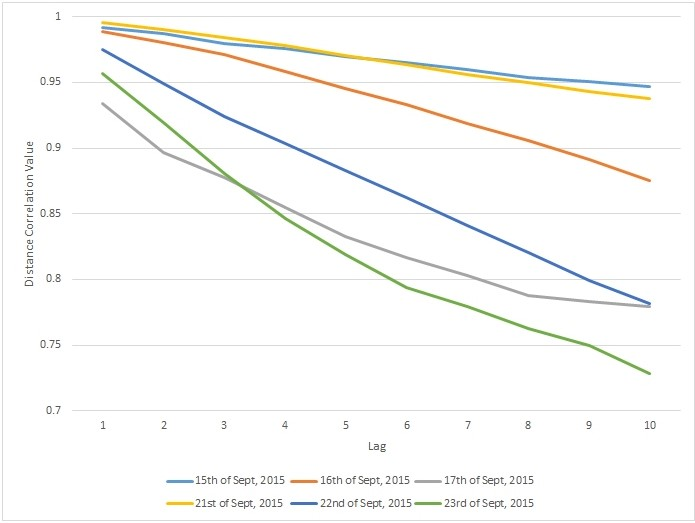
\includegraphics[width= 1\textwidth]{distancecorrelation}
\caption{Distance Correlation Values for Volkswagen Training Dataset}
\end{figure}

In the days before the official release of the news about Volkswagen's failure to meet regulations, the correlation values follow a generally decreasing order with respect to time passing in days, hence the correlation between previous prices and the current price decreases as the days approach the date of the official news release, the 18th of September 2015. This decrease in correlation indicates an increase in the volatility of prices as time increases, for example, on the 15th of September, the previous prices up to ten minutes in the past have a correlation of at least 0.95 with the current price, but by the 17th, even the price in the previous minute has less than 0.95 correlation with the current price. \par

Comparing the correlation values for the 15th of September and 21st of September, there is generally a higher correlation between prices in the previous five minutes and the current price on the 21st than the 15th. However, prices from six to ten minutes before the current price have a higher correlation with the current price on the 15th than on the 21st. This suggests that, recent prices that are further away in time are more relevant when predicting prices on the 15th than on the 21st; but prices that are closer to the current price in time are more useful for predicting the current price on the 21st than on the 15th. This could also indicate that there is a significant change in the behaviour of prices after approximately every five minutes  on the 21st; thus suggesting a cycle of stability in prices followed by increased volatility with respect to time.\par

After the official release of the news, there is a significant increase in the correlation values between recent prices and the current price; prices up to ten minutes before the current price are more correlated with the current price than on the last day before the release of the news, that is, 17th of September. This suggests that the behaviour of the price was less volatile on the last day before the news was released, than on the first day after the news was released; also indicating that prices were more stable and predictable on the 21st than on the 17th. However, between the 21st and 23rd of September, the correlation values gradually decrease, and the 23rd has the lowest correlation values measured in this experiment.

Based on the significance value of 0.945 which as part of the experiment's design, was chosen as the cut off for selecting a lagged variable to be used as a feature in the equation discovery task, table \ref{selectedfeaturestab} lists the features selected for each day. It is important to note that the 17th of September had no correlation values that satisfied this criteria, so the lagged variable with the highest correlation value has been selected; this is Lag 1.

\begin{table}[H]
\centering
\begin{tabular}{|l|l|}
\hline
           & \multicolumn{1}{c|}{Selected Features}                                \\ \hline
15/09/2015 & Lag 1, Lag 2, Lag 3, Lag 4, Lag 5, Lag 6, Lag 7, Lag 8, Lag 9, Lag 10 \\ \hline
16/09/2015 & Lag 1, Lag 2, Lag 3, Lag 4, Lag 5                                     \\ \hline
17/09/2015 & Lag 1                                                                 \\ \hline
21/09/2015 & Lag 1, Lag 2, Lag 3, Lag 4, Lag 5, Lag 6, Lag 7, Lag 8                \\ \hline
22/09/2015 & Lag 1, Lag 2                                                          \\ \hline
23/09/2015 & Lag 1                                                                 \\ \hline
\end{tabular}
\caption{Selected Features for Volkswagen Training Dataset}
\label{selectedfeaturestab}
\end{table}


\begin{table}[H]
\centering
\label{forddcvtab}
\begin{tabular}{|l|l|l|l|l|l|l|}
\hline
       & \multicolumn{3}{c|}{Before the News} & \multicolumn{3}{c|}{After the News}  \\ \hline
       & 15/09/2015 & 16/09/2015 & 17/09/2015 & 21/09/2015 & 22/09/2015 & 23/09/2015 \\ \hline
Lag 1  & 0.9907     & 0.9951     & 0.9793     & 0.9467     & 0.9679     & 0.9668     \\ \hline
Lag 2  & 0.9848     & 0.9913     & 0.9637     & 0.9161     & 0.9388     & 0.9347     \\ \hline
Lag 3  & 0.9799     & 0.9876     & 0.953      & 0.88       & 0.9085     & 0.9112     \\ \hline
Lag 4  & 0.9762     & 0.985      & 0.9429     & 0.8476     & 0.8825     & 0.8936     \\ \hline
Lag 5  & 0.9712     & 0.9824     & 0.9356     & 0.8169     & 0.8585     & 0.8801     \\ \hline
Lag 6  & 0.9646     & 0.9786     & 0.9216     & 0.7907     & 0.8325     & 0.8619     \\ \hline
Lag 7  & 0.9582     & 0.9748     & 0.9066     & 0.7657     & 0.807      & 0.8378     \\ \hline
Lag 8  & 0.955      & 0.9703     & 0.8959     & 0.7411     & 0.7802     & 0.8081     \\ \hline
Lag 9  & 0.952      & 0.9661     & 0.8887     & 0.722      & 0.755      & 0.7807     \\ \hline
Lag 10 & 0.9484     & 0.9623     & 0.8798     & 0.7103     & 0.7357     & 0.7558     \\ \hline
\end{tabular}
\caption{Distance Correlation Values for Ford Training Dataset}
\end{table}

\begin{figure}[H]
\centering
\label{forddcvfig}
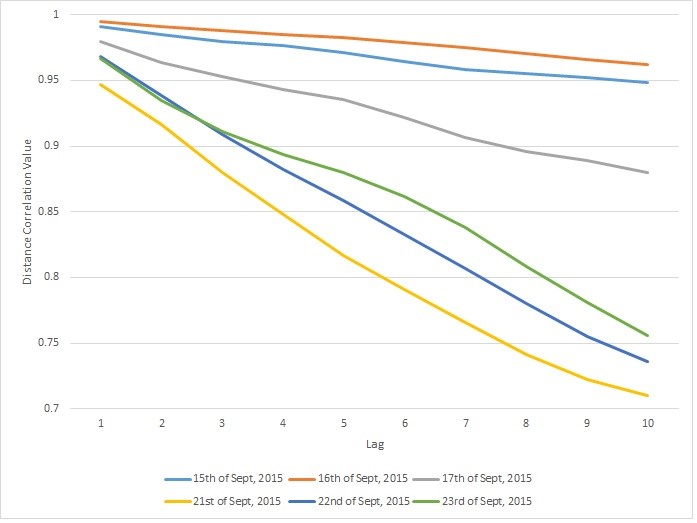
\includegraphics[width= 1\textwidth]{ford_distancecorrelation}
\caption{Distance Correlation Values for Ford Training Dataset}
\end{figure}

\section{Equation Discovery}
\subsection{15th of September 2015}
\paragraph{Linear equations}\hfill \break
summary ...
\begin{equation} 
close_{t} = 0.0493762 + 0.998771 * close_{t-1} + -0.191399 * close_{t-3} + 0.183886 * close_{t-4} 
\label{Equation 5.1}
\end{equation}
\begin{equation} 
close_{t} = 0.0473247 + 0.108798 * close_{t-4} + 0.934382 * close_{t-1} + -0.0518387 * close_{t-6}  
\label{Equation 5.2}
\end{equation}

\begin{table}[H]
\centering

\label{linear15tab}
\begin{tabular}{|l|l|l|l|}
\hline
\textbf{Dataset}                   & \textbf{Measure} & \textbf{\begin{tabular}[c]{@{}l@{}}Best Equation for \\ Training Set (Equation 5.1)\end{tabular}} & \textbf{\begin{tabular}[c]{@{}l@{}}Best Equation for\\ Test Set (Equation 5.2)\end{tabular}} \\ \hline
\multirow{4}{*}{\textit{Test set}} & MSE              & 0.0017898                                                                                         & 0.0017393                                                                                    \\ \cline{2-4} 
                                   & RMSE             & 0.0423058                                                                                         & 0.0417053                                                                                    \\ \cline{2-4} 
                                   & MFE              & -0.0045250                                                                                        & -0.0030887                                                                                   \\ \cline{2-4} 
                                   & MAD              & 0.0209052                                                                                         & 0.0214432                                                                                    \\ \hline
\textit{Training set}              & MSE              & 0.0105372                                                                                         & 0.0107417                                                                                    \\ \hline
\end{tabular}
\caption{Linear function results summary of best equations for the 15th of September, 2015}
\end{table}

\begin{figure}[H]
\centering
\label{VWlinear15fig}
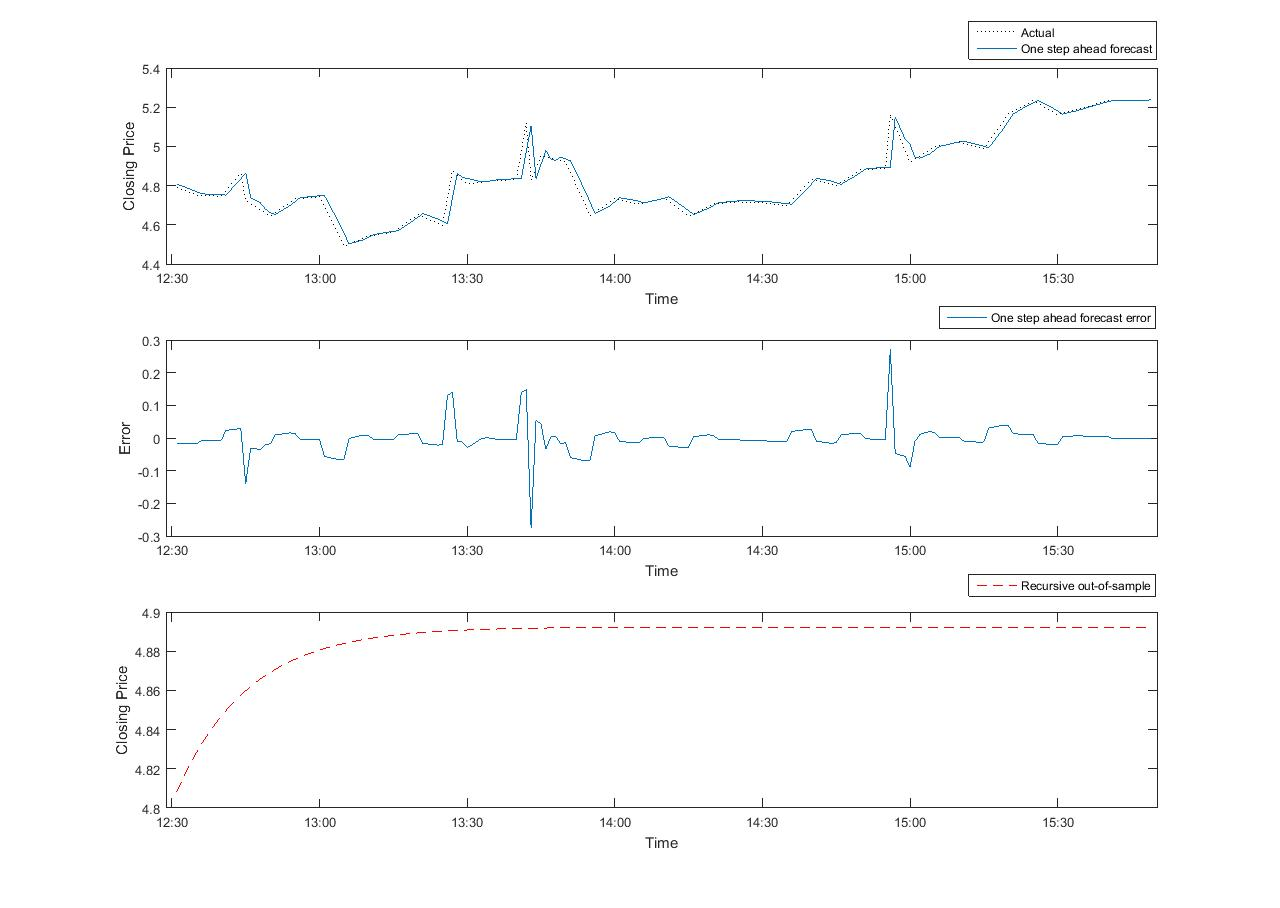
\includegraphics[width=\textwidth]{15linear2}
\caption{Top: Time plot of linear model \ref{Equation 5.2} one-step forecast vs. actual values for the 15th of September. Middle: Error value for each time point. Bottom: Time plot of recursive out-of-sample forecast using model \ref{Equation 5.2}}
\end{figure}

\paragraph{Sine function equations}\hfill \break
summary ...
\begin{equation}
\begin{align*}
 close_{t} = 0.146912 + 0.962927 * close_{t-1} + 0.558971 * close_{t-2} *sin ( -2.30527 * close_{t-10} + 7.42028 ) \\+0.564857
             *close_{t-1} * sin ( 2.28032 * close_{t-10} + -7.31432 )   
\end{align*}
\label{Equation 5.3}
\end{equation}

\begin{equation}
\begin{align*}
close_{t} = 1.00846 * close_{t-1} + -0.628636 * close_{t-1} * sin ( -2.15488 * close_{t-10} + 7.0329 ) + 0.631036
\\ * close_{t-2} * sin ( -2.15326 * close_{t-10} + 7.04004 )
\end{align*}
\label{Equation 5.4}
\end{equation}

\begin{table}[H]
\centering

\label{nonlinear15tab}
\begin{tabular}{|l|l|l|l|}
\hline
\textbf{Dataset}                   & \textbf{Measure} & \textbf{\begin{tabular}[c]{@{}l@{}}Best Equation for \\ Training Set (Equation 5.3)\end{tabular}} & \textbf{\begin{tabular}[c]{@{}l@{}}Best Equation for\\ Test Set (Equation 5.4)\end{tabular}} \\ \hline
\multirow{4}{*}{\textit{Test set}} & MSE              & 0.0026621                                                                                         & 0.0018205                                                                                    \\ \cline{2-4} 
                                   & RMSE             & 0.0515951                                                                                         & 0.0426672                                                                                    \\ \cline{2-4} 
                                   & MFE              & 0.0211936                                                                                         & 0.0001406                                                                                    \\ \cline{2-4} 
                                   & MAD              & 0.0341720                                                                                         & 0.0230330                                                                                    \\ \hline
\textit{Training set}              & MSE              & 0.0088404                                                                                         & 0.0093408                                                                                    \\ \hline
\end{tabular}
\caption{Sine function results summary of best equations for the 15th of September, 2015}
\end{table}

\begin{figure}[H]
\centering
\label{VWNonlinear15fig}
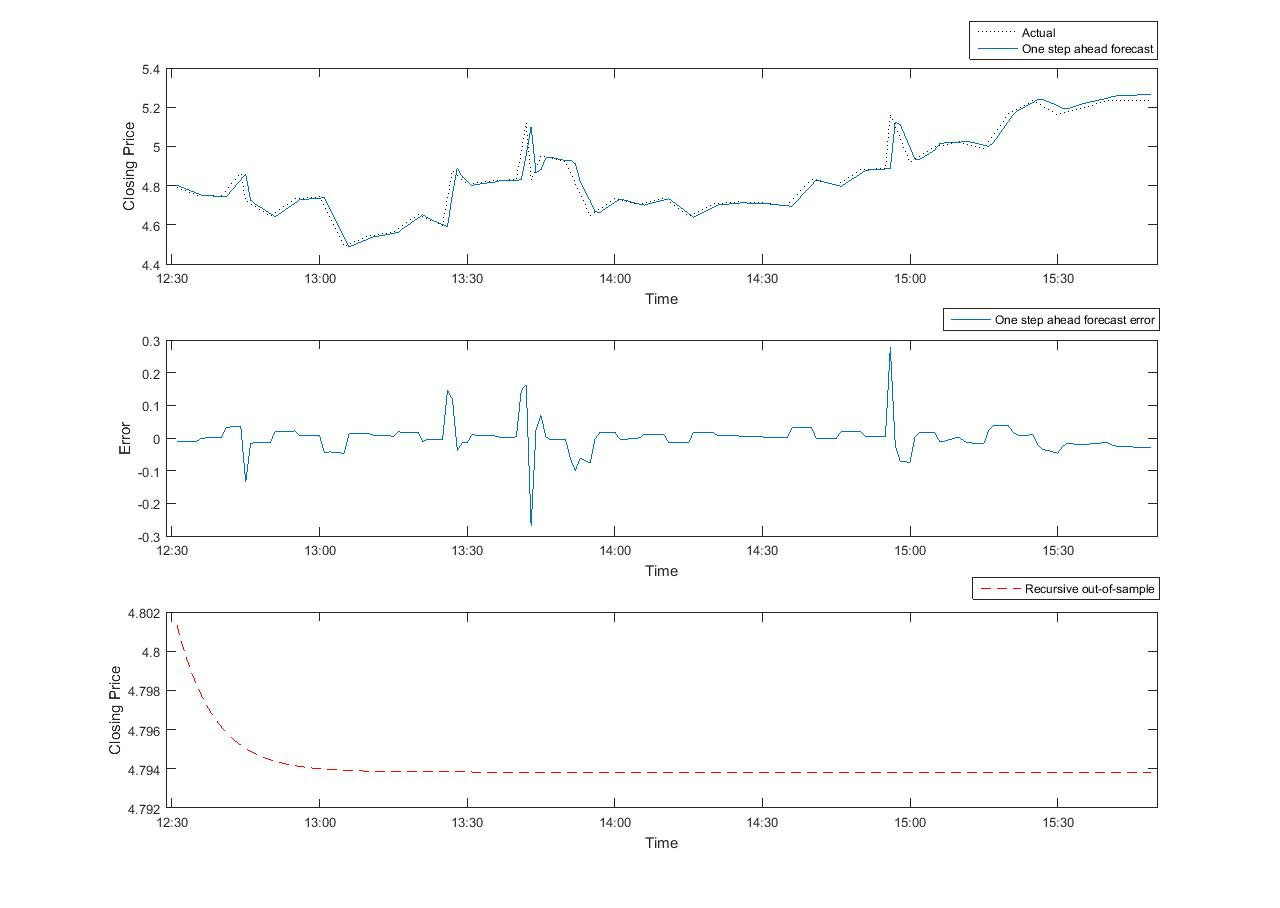
\includegraphics[width=\textwidth]{15nonlinear}
\caption{Top: Time plot of sine function model \ref{Equation 5.4} one-step forecast vs. actual values for the 15th of September. Middle: Error value for each time point. Bottom: Time plot of recursive out-of-sample forecast using model \ref{Equation 5.4}}
\end{figure}

\subsection{16th of September 2015}
\paragraph{Linear equations}\hfill \break
summary ...

\begin{equation}
\begin{align*}
close_{t} = 0.0580705 + 0.994127 * close_{t-1} + 0.0614415 * close_{t-6} + -0.060513 * close_{t-9}
\end{align*}
\label{Equation 5.5}
\end{equation}
\begin{equation}
\begin{align*}
close_{t} = 0.0566784 + 0.0794151 * close_{t-8} + 1.00662 * close_{t-1} + -0.0908324 * close_{t-9}
\end{align*}
\label{Equation 5.6}
\end{equation}

\begin{table}[H]
\centering
\label{linear16tab}
\begin{tabular}{|l|l|l|l|}
\hline
\textbf{Dataset}                   & \textbf{Measure} & \textbf{\begin{tabular}[c]{@{}l@{}}Best Equation for \\ Training Set (Equation 5.5)\end{tabular}} & \textbf{\begin{tabular}[c]{@{}l@{}}Best Equation for\\ Test Set (Equation 5.6)\end{tabular}} \\ \hline
\multirow{4}{*}{\textit{Test set}} & MSE              & 0.0014666                                                                                         & 0.0014211                                                                                    \\ \cline{2-4} 
                                   & RMSE             & 0.0382968                                                                                         & 0.0376976                                                                                    \\ \cline{2-4} 
                                   & MFE              & 0.0020208                                                                                         & 0.0017421                                                                                    \\ \cline{2-4} 
                                   & MAD              & 0.0225442                                                                                         & 0.0220749                                                                                    \\ \hline
\textit{Training set}              & MSE              & 0.0085253                                                                                        & 0.0085355                                                                                    \\ \hline
\end{tabular}
\caption{Linear function results summary of best equations for the 16th of September, 2015}
\end{table}

\begin{figure}[H]
\centering
\label{VWlinear16fig}
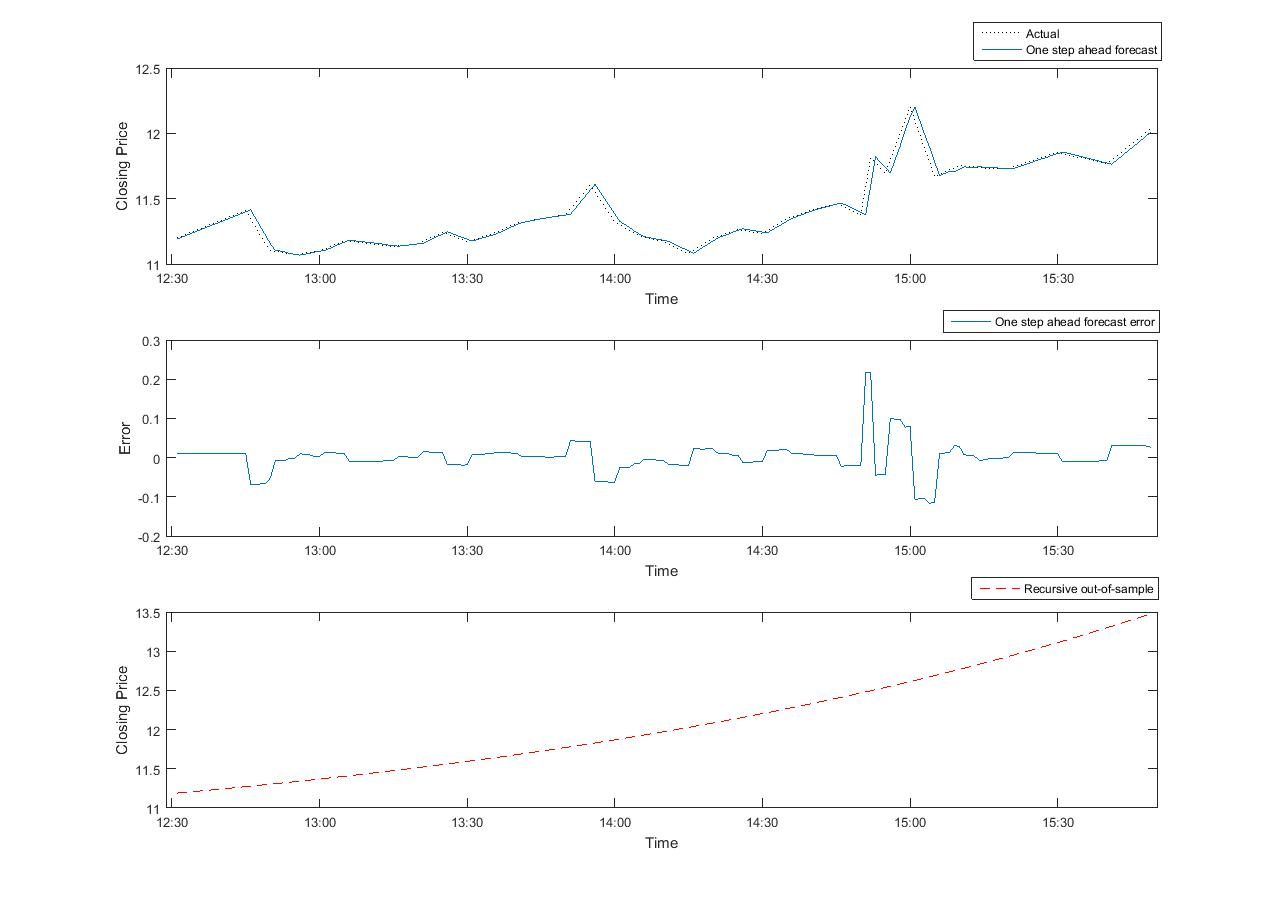
\includegraphics[width=\textwidth]{16linear2}
\caption{Top: Time plot of linear model \ref{Equation 5.6} one-step forecast vs. actual values for the 16th of September. Middle: Error value for each time point. Bottom: Time plot of recursive out-of-sample forecast using model \ref{Equation 5.6}}
\end{figure}

\paragraph{Sine function equations}\hfill \break
summary ...
\begin{equation}
\begin{align*}
close_{t} = 0.191979 + 0.935382 * close_{t-1} + 0.0600035 * close_{t-9} * sin ( -1.01091 * close_{t-2} + 7.3806 ) + -0.102636\\ * close_{t-2} * sin ( -0.673581 * close_{t-2} + 4.38998 )
\end{align*}
\label{Equation 5.7}
\end{equation}

\begin{equation}
\begin{align*}
close_{t} = 9.8704 + -0.0474591 * close_{t-10} + -0.319492 * close_{t-4} * sin ( -0.313859 * close_t-1 + 3.03459 ) + \\-0.0314043 * close_{t-8} * sin ( -0.958882 * close_{t-2} + 8.07974 )
\end{align*}
\label{Equation 5.8}
\end{equation}

\begin{table}[H]
\centering
\label{nonlinear16tab}
\begin{tabular}{|l|l|l|l|}
\hline
\textbf{Dataset}                   & \textbf{Measure} & \textbf{\begin{tabular}[c]{@{}l@{}}Best Equation for \\ Training Set (Equation 5.7)\end{tabular}} & \textbf{\begin{tabular}[c]{@{}l@{}}Best Equation for\\ Test Set (Equation 5.8)\end{tabular}} \\ \hline
\multirow{4}{*}{\textit{Test set}} & MSE              & 0.0519552                                                                                         & 0.0155245                                                                                    \\ \cline{2-4} 
                                   & RMSE             & 0.2279368                                                                                         & 0.1245975                                                                                    \\ \cline{2-4} 
                                   & MFE              & 0.1750767                                                                                         & 0.0988577                                                                                    \\ \cline{2-4} 
                                   & MAD              & 0.1750767                                                                                         & 0.0992733                                                                                    \\ \hline
\textit{Training set}              & MSE              & 0.0080155                                                                                         & 0.0080263                                                                                    \\ \hline
\end{tabular}
\caption{Sine function results summary of best equations for the 16th of September, 2015}
\end{table}

\begin{figure}[H]
\centering
\label{VWNonlinear16fig}
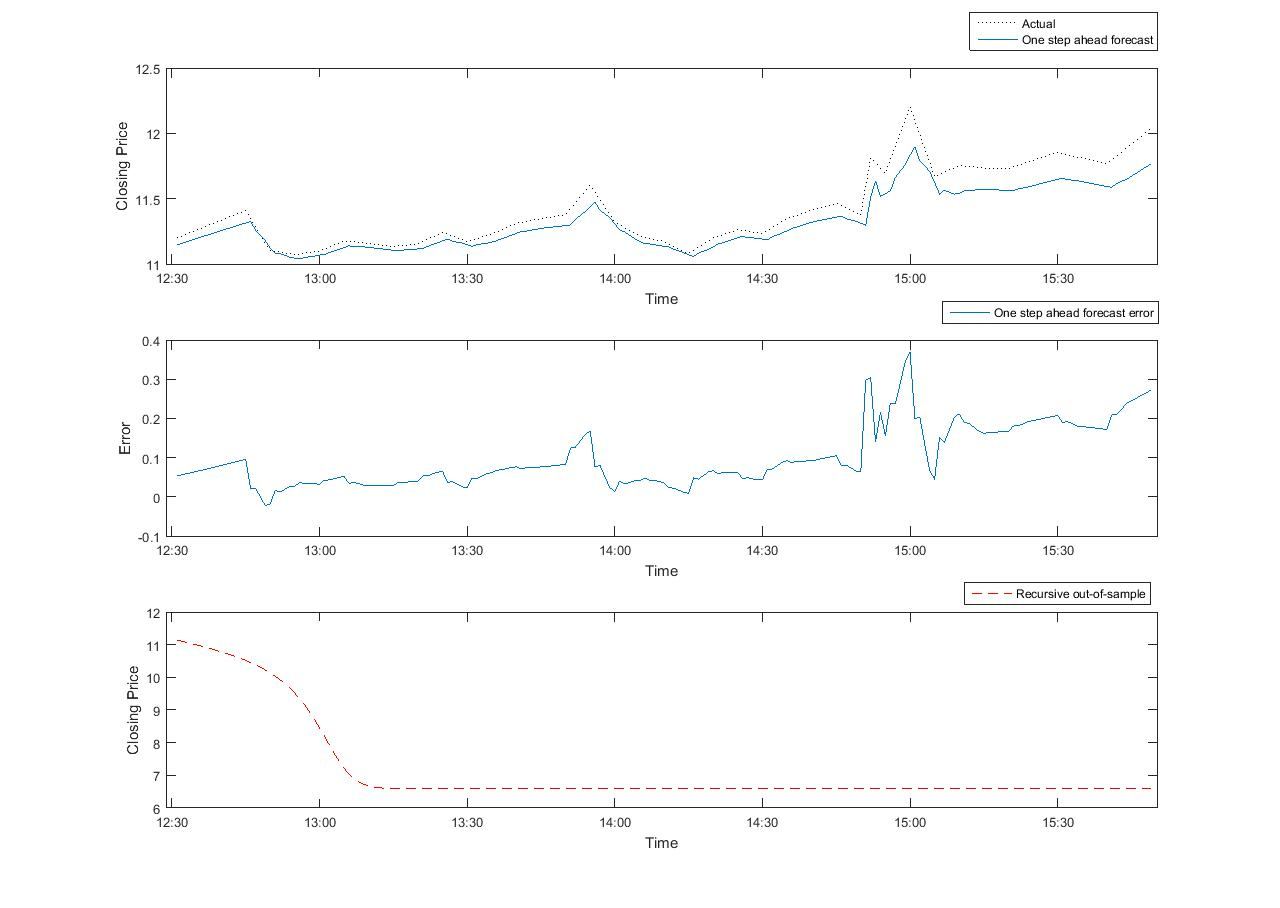
\includegraphics[width=\textwidth]{16nonlinear}
\caption{Top: Time plot of sine function model \ref{Equation 5.8} one-step forecast vs. actual values for the 16th of September. Middle: Error value for each time point. Bottom: Time plot of recursive out-of-sample forecast using model \ref{Equation 5.8}}
\end{figure}

\subsection{17th of September 2015}
\paragraph{Linear equations}\hfill \break
summary ...

\begin{equation}
\begin{align*}
close_{t} = 1.05318 + 0.873188 * close_{t-1} + 0.1384 * close_{t-3} + -0.0808047 * close_{t-4} 
\end{align*}
\label{Equation 5.9}
\end{equation}
\begin{equation}
\begin{align*}
close_{t} = 1.05318 + 0.873188 * close_{t-1} + 0.1384 * close_{t-3} + -0.0808047 * close_{t-4} 
\end{align*}
\label{Equation 5.10}
\end{equation}

\begin{table}[H]
\centering
\begin{tabular}{|l|l|l|l|}
\hline
\textbf{Dataset}                   & \textbf{Measure} & \textbf{\begin{tabular}[c]{@{}l@{}}Best Equation for \\ Training Set (Equation 5.9)\end{tabular}} & \textbf{\begin{tabular}[c]{@{}l@{}}Best Equation for\\ Test Set (Equation 5.10)\end{tabular}} \\ \hline
\multirow{4}{*}{\textit{Test set}} & MSE              & 0.0071149                                                                                         & 0.0071149                                                                                     \\ \cline{2-4} 
                                   & RMSE             & 0.0843500                                                                                         & 0.0843500                                                                                     \\ \cline{2-4} 
                                   & MFE              & 0.0310073                                                                                         & 0.0310073                                                                                     \\ \cline{2-4} 
                                   & MAD              & 0.0563057                                                                                         & 0.0563057                                                                                     \\ \hline
\textit{Training set}              & MSE              & 0.0032743                                                                                         & 0.0032743                                                                                     \\ \hline
\end{tabular}
\caption{Linear function results summary of best equations for the 17th of September, 2015}
\label{linear17tab}
\end{table}

\begin{figure}[H]
\centering
\label{VWlinear17fig}
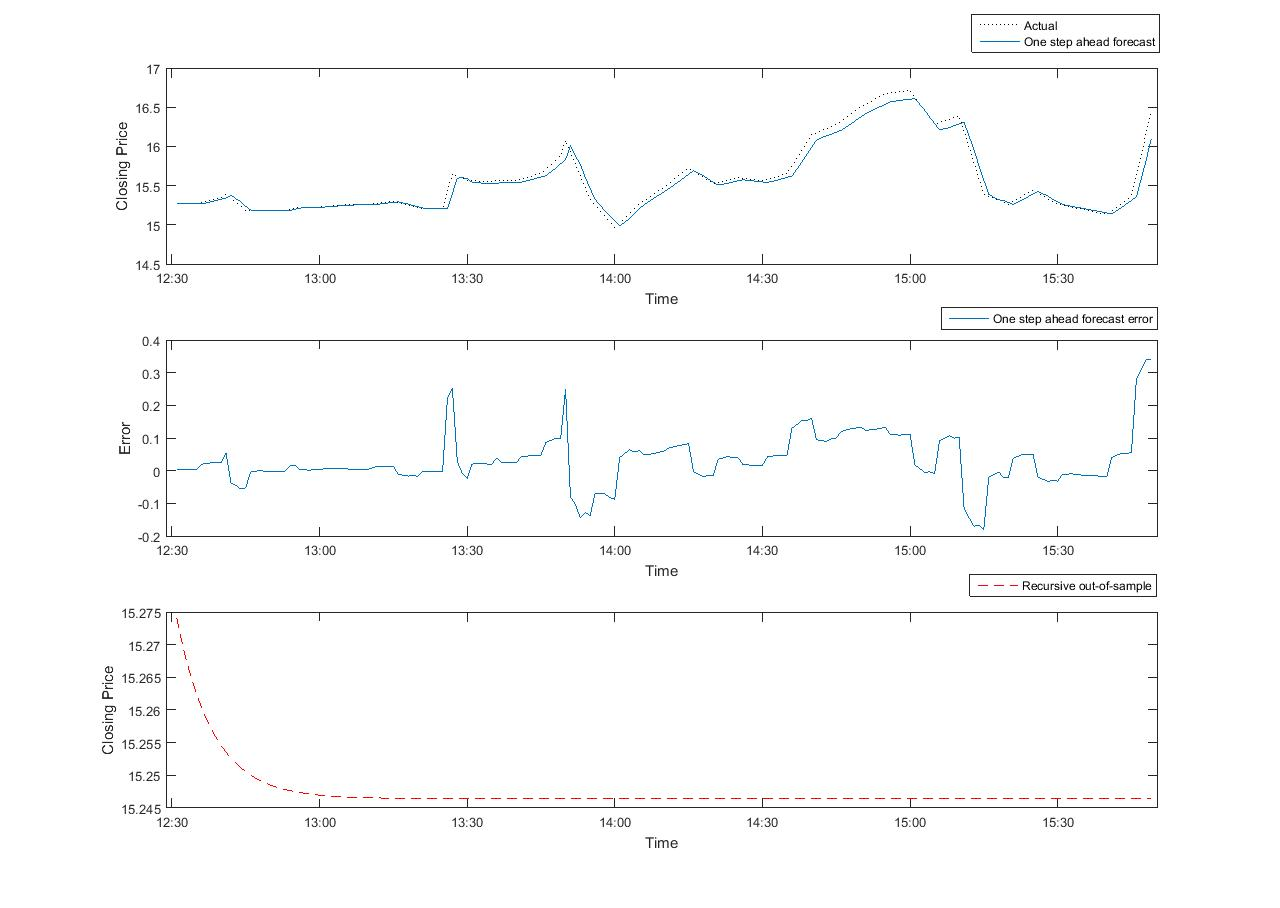
\includegraphics[width=\textwidth]{17linear2}
\caption{Top: Time plot of linear model \ref{Equation 5.10} one-step forecast vs. actual values for the 17th of September. Middle: Error value for each time point. Bottom: Time plot of recursive out-of-sample forecast using model \ref{Equation 5.10}}
\end{figure}

\paragraph{Sine function equations}\hfill \break
summary ...
\begin{equation}
\begin{align*}
close_{t} = 9.77018 + 5.25977 + 0.0740164 * close_{t-1} * sin ( -0.83872 * close_{t-1} + -3.10999 ) + 0.0242214\\ * sin ( -6.84365 * close_{t-7} + 10 ) 
\end{align*}
\label{Equation 5.11}
\end{equation}

\begin{equation}
\begin{align*}
close_{t} = 7.79615 + 7.18875 + 0.0350744 * sin ( 4.7513 * close_{t-9} + -7.35244 ) + 0.0862542 * close_{t-2} \\ * sin ( -0.672662 * close_{t-1} + -5.63082 )
\end{align*}
\label{Equation 5.12}
\end{equation}

\begin{table}[H]
\centering
\begin{tabular}{|l|l|l|l|}
\hline
\textbf{Dataset}                   & \textbf{Measure} & \textbf{\begin{tabular}[c]{@{}l@{}}Best Equation for \\ Training Set (Equation 5.11)\end{tabular}} & \textbf{\begin{tabular}[c]{@{}l@{}}Best Equation for\\ Test Set (Equation 5.12)\end{tabular}} \\ \hline
\multirow{4}{*}{\textit{Test set}} & MSE              & 0.0220058                                                                                          & 0.0213008                                                                                     \\ \cline{2-4} 
                                   & RMSE             & 0.1483435                                                                                          & 0.1459480                                                                                     \\ \cline{2-4} 
                                   & MFE              & 0.0742246                                                                                          & 0.0836738                                                                                     \\ \cline{2-4} 
                                   & MAD              & 0.0907257                                                                                          & 0.0963079                                                                                     \\ \hline
\textit{Training set}              & MSE              & 0.0031259                                                                                          & 0.0031642                                                                                     \\ \hline
\end{tabular}
\caption{Sine function results summary of best equations for the 17th of September, 2015}
\label{nonlinear17tab}
\end{table}

\begin{figure}[H]
\centering
\label{VWNonlinear17fig}
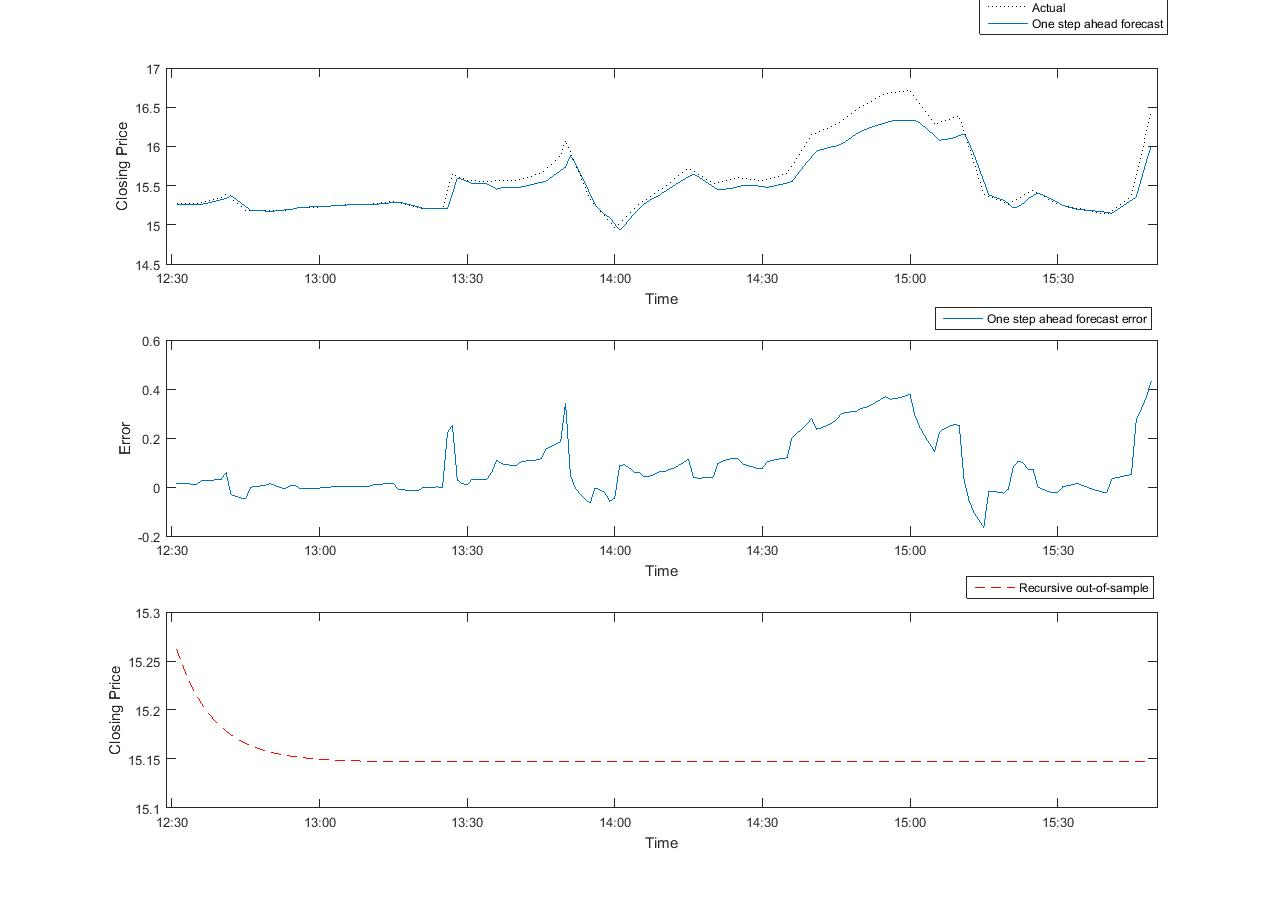
\includegraphics[width=\textwidth]{17nonlinear}
\caption{Top: Time plot of sine function model \ref{Equation 5.12} one-step forecast vs. actual values for the 17th of September. Middle: Error value for each time point. Bottom: Time plot of recursive out-of-sample forecast using model \ref{Equation 5.12}}
\end{figure}


\subsection{18th of September 2015}
\paragraph{Linear equations}\hfill \break
summary ...
\begin{equation}
\begin{align*}
close_{t} = 0.241257 + 1.03807 * close_{t-1} + -0.107004 * close_{t-4} + 0.0543023 * close_{t-7} 
\end{align*}
\label{Equation 5.13}
\end{equation}
\begin{equation}
\begin{align*}
 close_{t} = 0.23453 + 1.03379 * close_{t-1} + -0.0830913 * close_{t-4} + 0.0351304 * close_{t-10} 
\end{align*}
\label{Equation 5.14}
\end{equation}

\begin{table}[H]
\centering
\begin{tabular}{|l|l|l|l|}
\hline
\textbf{Dataset}                   & \textbf{Measure} & \textbf{\begin{tabular}[c]{@{}l@{}}Best Equation for \\ Training Set (Equation 5.13)\end{tabular}} & \textbf{\begin{tabular}[c]{@{}l@{}}Best Equation for\\ Test Set (Equation 5.14)\end{tabular}} \\ \hline
\multirow{4}{*}{\textit{Test set}} & MSE              & 0.0041244                                                                                          & 0.0039525                                                                                     \\ \cline{2-4} 
                                   & RMSE             & 0.0642215                                                                                          & 0.0628693                                                                                     \\ \cline{2-4} 
                                   & MFE              & -0.0064098                                                                                         & -0.0074246                                                                                    \\ \cline{2-4} 
                                   & MAD              & 0.0376043                                                                                          & 0.0365190                                                                                     \\ \hline
\textit{Training set}              & MSE              & 0.0161145                                                                                          & 0.0161382                                                                                     \\ \hline
\end{tabular}
\caption{Linear function results summary of best equations for the 18th of September, 2015}
\label{linear18tab}
\end{table}

\begin{figure}[H]
\centering
\label{VWlinear18fig}
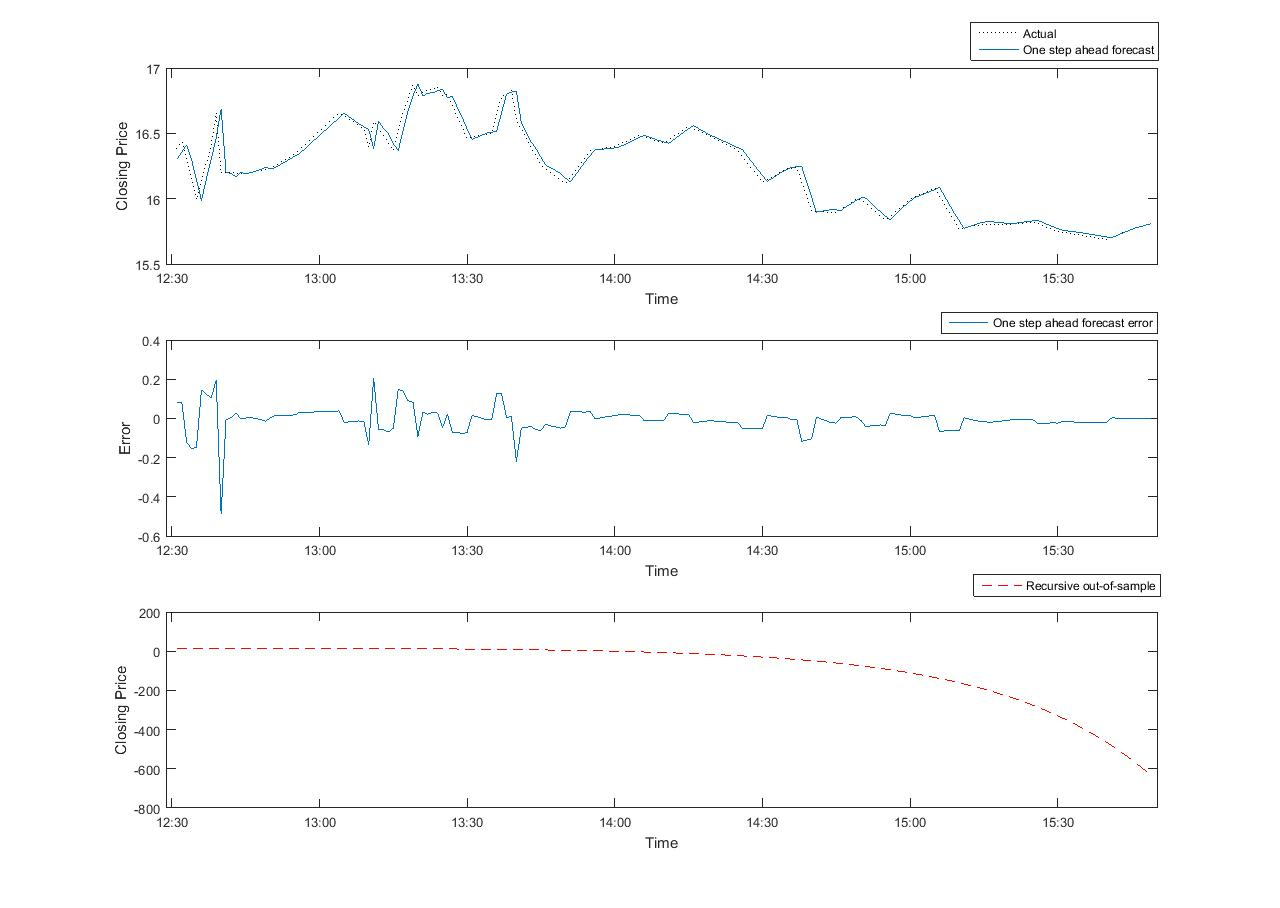
\includegraphics[width=\textwidth]{18linear}
\caption{Top: Time plot of linear model \ref{Equation 5.14} one-step forecast vs. actual values for the 18th of September. Middle: Error value for each time point. Bottom: Time plot of recursive out-of-sample forecast using model \ref{Equation 5.14}}
\end{figure}

\paragraph{Sine function equations}\hfill \break
summary ...
\begin{equation}
\begin{align*}
close_{t} = -1.44783 + 0.1436 * close_{t-7} + -0.0939442 * close_{t-8} * sin ( 0.4082 * close_{t-5} + -4.90259 ) \\+ 1.04462 * close_{t-1} * sin ( 0.127987 * close_{t-4} + -0.404009 )
\end{align*}
\label{Equation 5.15}
\end{equation}

\begin{equation}
\begin{align*}
 close_{t} = -0.49966 + 0.0677348 * close_{t-10} + 1.03712 * close_{t-1} * sin ( 0.129323 * close_{t-4} + -0.424887 )\\ + -0.0708436 * close_{t-8} * sin ( 0.46844 * close_{t-5} + -5.73401 )
\end{align*}
\label{Equation 5.16}
\end{equation}

\begin{table}[H]
\centering
\begin{tabular}{|l|l|l|l|}
\hline
\textbf{Dataset}                   & \textbf{Measure} & \textbf{\begin{tabular}[c]{@{}l@{}}Best Equation for \\ Training Set (Equation 5.15)\end{tabular}} & \textbf{\begin{tabular}[c]{@{}l@{}}Best Equation for\\ Test Set (Equation 5.16)\end{tabular}} \\ \hline
\multirow{4}{*}{\textit{Test set}} & MSE              & 0.0046094                                                                                          & 0.0042209                                                                                     \\ \cline{2-4} 
                                   & RMSE             & 0.0678927                                                                                          & 0.0649684                                                                                     \\ \cline{2-4} 
                                   & MFE              & -0.0113059                                                                                         & -0.0141285                                                                                    \\ \cline{2-4} 
                                   & MAD              & 0.0414024                                                                                          & 0.0402060                                                                                     \\ \hline
\textit{Training set}              & MSE              & 0.0152577                                                                                          & 0.0153097                                                                                     \\ \hline
\end{tabular}
\caption{Sine function results summary of best equations for the 18th of September, 2015}
\label{nonlinear18tab}
\end{table}

\begin{figure}[H]
\centering
\label{VWNonlinear18fig}
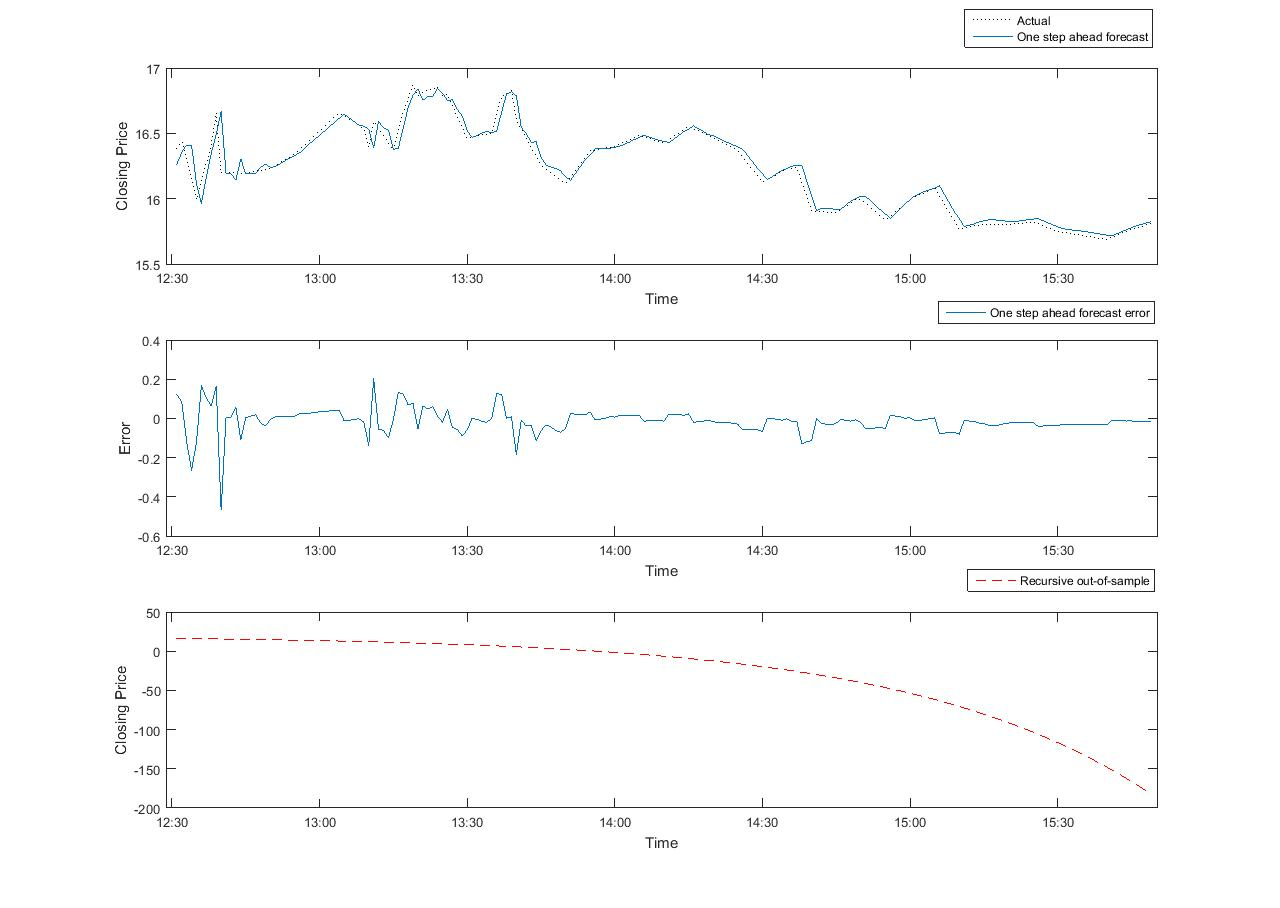
\includegraphics[width= \textwidth]{18nonlinear}
\caption{Top: Time plot of sine function model \ref{Equation 5.16} one-step forecast vs. actual values for the 18th of September. Middle: Error value for each time point. Bottom: Time plot of recursive out-of-sample forecast using model \ref{Equation 5.16}}
\end{figure}



\subsection{21st of September 2015}
\paragraph{Linear equations}\hfill \break
summary ...
\begin{equation}
\begin{align*}
close_{t} = -0.0128103 + 0.0879563 * close_{t-8} + 1.04437 * close_{t-1} + -0.1366 * close_{t-6}
\end{align*}
\label{Equation 5.17}
\end{equation}
\begin{equation}
\begin{align*}
close_{t} = -0.0109011 + 0.064052 * close_{t-9} + -0.110824 * close_{t-6} + 1.04264 * close_{t-1}
\end{align*}
\label{Equation 5.18}
\end{equation}

\begin{table}[H]
\centering
\begin{tabular}{|l|l|l|l|}
\hline
\textbf{Dataset}                   & \textbf{Measure} & \textbf{\begin{tabular}[c]{@{}l@{}}Best Equation for \\ Training Set (Equation 5.17)\end{tabular}} & \textbf{\begin{tabular}[c]{@{}l@{}}Best Equation for\\ Test Set (Equation 5.18)\end{tabular}} \\ \hline
\multirow{4}{*}{\textit{Test set}} & MSE              & 0.0203478                                                                                          & 0.0202285                                                                                     \\ \cline{2-4} 
                                   & RMSE             & 0.1426457                                                                                          & 0.1422270                                                                                     \\ \cline{2-4} 
                                   & MFE              & -0.0000889                                                                                         & -0.0010640                                                                                    \\ \cline{2-4} 
                                   & MAD              & 0.0859956                                                                                          & 0.0863261                                                                                     \\ \hline
\textit{Training set}              & MSE              & 0.0295856                                                                                          & 0.0296586                                                                                     \\ \hline
\end{tabular}
\caption{Linear function results summary of best equations for the 21st of September, 2015}
\label{linear21tab}
\end{table}

\begin{figure}[H]
\centering
\label{VWlinear21fig}
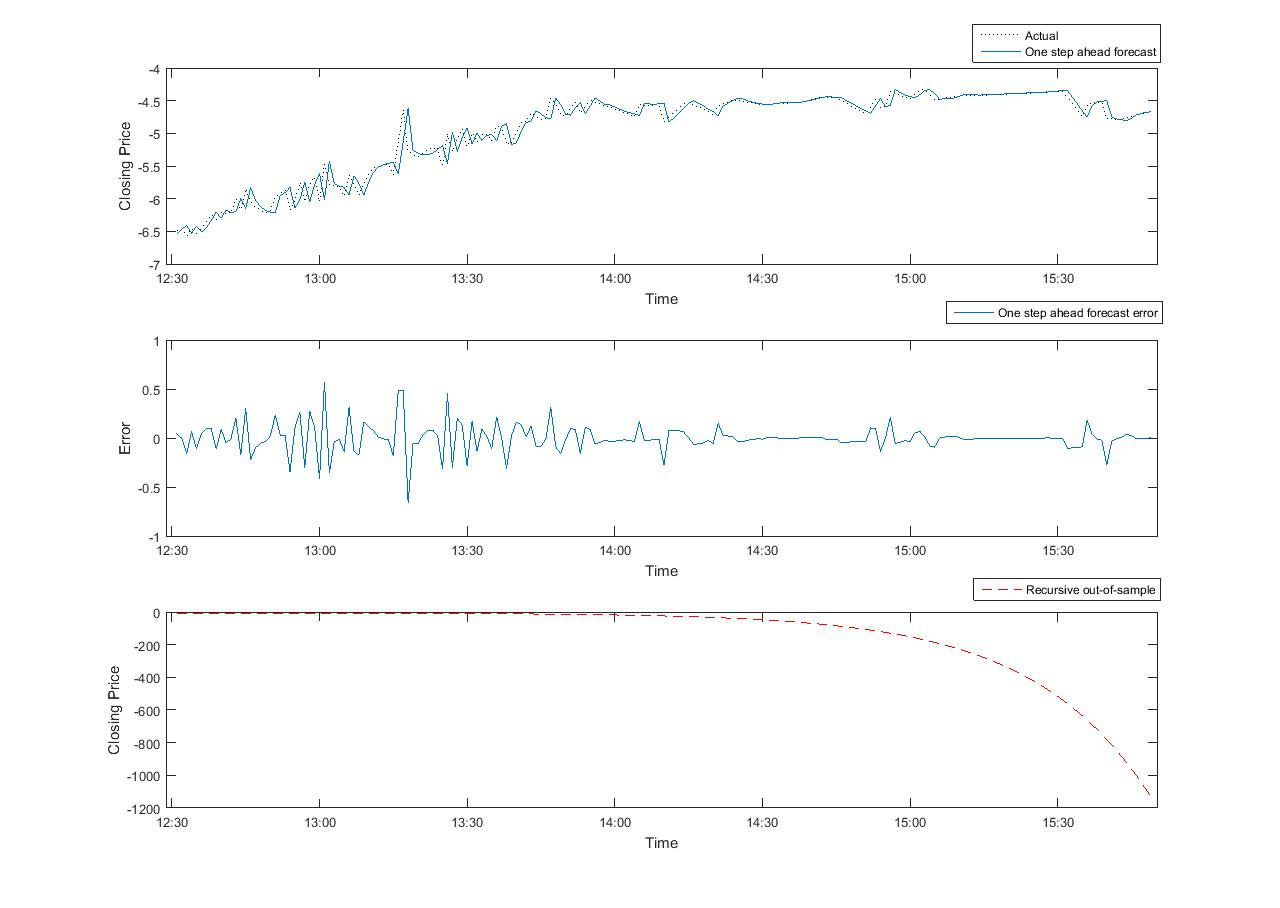
\includegraphics[width=\textwidth]{21linear}
\caption{Top: Time plot of linear model \ref{Equation 5.18} one-step forecast vs. actual values for the 21st of September. Middle: Error value for each time point. Bottom: Time plot of recursive out-of-sample forecast using model \ref{Equation 5.18}}
\end{figure}

\paragraph{Sine function equations}\hfill \break
summary ...
\begin{equation}
\begin{align*}
close_{t} = -3.25786 + 0.568724 * close_{t-1} + -0.121701 * close_{t-10} * sin ( 0.533977 * close_{t-1} + 4.19195 ) + \\ -0.201465 * sin ( -1.54106 * close_{t-4} + -10 ) 
\end{align*}
\label{Equation 5.19}
\end{equation}

\begin{equation}
\begin{align*}
close_{t} = -1.36096 + 0.825838 * close_{t-1} + -0.186701 * sin ( -1.5409 * close_t-4 + -10 ) + -0.0456466 \\ * close_{t-9} * sin ( 0.812868 * close_{t-1} + 6.71715 )
\end{align*}
\label{Equation 5.20}
\end{equation}

\begin{table}[H]
\centering
\begin{tabular}{|l|l|l|l|}
\hline
\textbf{Dataset}                   & \textbf{Measure} & \textbf{\begin{tabular}[c]{@{}l@{}}Best Equation for \\ Training Set (Equation 5.19)\end{tabular}} & \textbf{\begin{tabular}[c]{@{}l@{}}Best Equation for\\ Test Set (Equation 5.20)\end{tabular}} \\ \hline
\multirow{4}{*}{\textit{Test set}} & MSE              & 0.3645990                                                                                          & 0.1937897                                                                                     \\ \cline{2-4} 
                                   & RMSE             & 0.6038204                                                                                          & 0.4402155                                                                                     \\ \cline{2-4} 
                                   & MFE              & 0.4900915                                                                                          & 0.3512108                                                                                     \\ \cline{2-4} 
                                   & MAD              & 0.5336193                                                                                          & 0.3939091                                                                                     \\ \hline
\textit{Training set}              & MSE              & 0.0242058                                                                                          & 0.0251018                                                                                     \\ \hline
\end{tabular}
\caption{Sine function results summary of best equations for the 21st of September, 2015}
\label{nonlinear21tab}
\end{table}

\begin{figure}[H]
\centering
\label{VWNonlinear21fig}
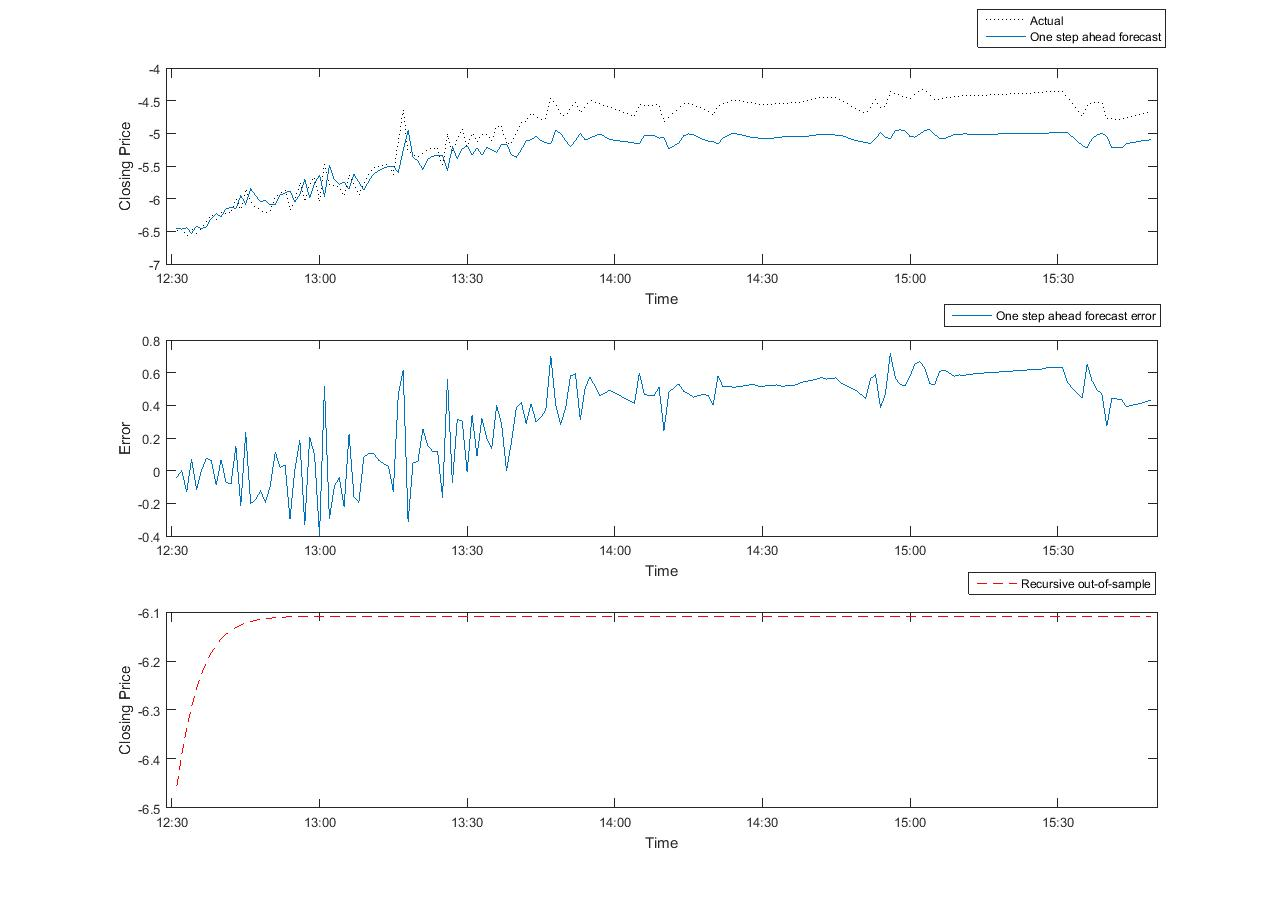
\includegraphics[width=\textwidth]{21nonlinear}
\caption{Top: Time plot of sine function model \ref{Equation 5.20} one-step forecast vs. actual values for the 21st of September. Middle: Error value for each time point. Bottom: Time plot of recursive out-of-sample forecast using model \ref{Equation 5.20}}
\end{figure}


\subsection{22nd of September 2015}
\paragraph{Linear equations}\hfill \break
summary ...
\begin{equation}
\begin{align*}
close_{t} = -1.04303 + 1.06684 * close_{t-1} + -0.0266356 * close_{t-9} + -0.0843253 * close_{t-2}
\end{align*}
\label{Equation 5.21}
\end{equation}
\begin{equation}
\begin{align*}
close_{t} = -0.920711 + -0.0221668 * close_{t-6} + 1.06944 * close_{t-1} + -0.086344 * close_{t-2}
\end{align*}
\label{Equation 5.22}
\end{equation}

\begin{table}[H]
\centering
\begin{tabular}{|l|l|l|l|}
\hline
\textbf{Dataset}                   & \textbf{Measure} & \textbf{\begin{tabular}[c]{@{}l@{}}Best Equation for \\ Training Set (Equation 5.21)\end{tabular}} & \textbf{\begin{tabular}[c]{@{}l@{}}Best Equation for\\ Test Set (Equation 5.22)\end{tabular}} \\ \hline
\multirow{4}{*}{\textit{Test set}} & MSE              & 0.0402115                                                                                          & 0.0356842                                                                                     \\ \cline{2-4} 
                                   & RMSE             & 0.2005279                                                                                          & 0.1889026                                                                                     \\ \cline{2-4} 
                                   & MFE              & 0.1401722                                                                                          & 0.1225137                                                                                     \\ \cline{2-4} 
                                   & MAD              & 0.1708389                                                                                          & 0.1563354                                                                                     \\ \hline
\textit{Training set}              & MSE              & 0.0622849                                                                                          & 0.0624398                                                                                     \\ \hline
\end{tabular}
\caption{Linear function results summary of best equations for the 22nd of September, 2015}
\label{linear22tab}
\end{table}

\begin{figure}[H]
\centering
\label{VWlinear22fig}
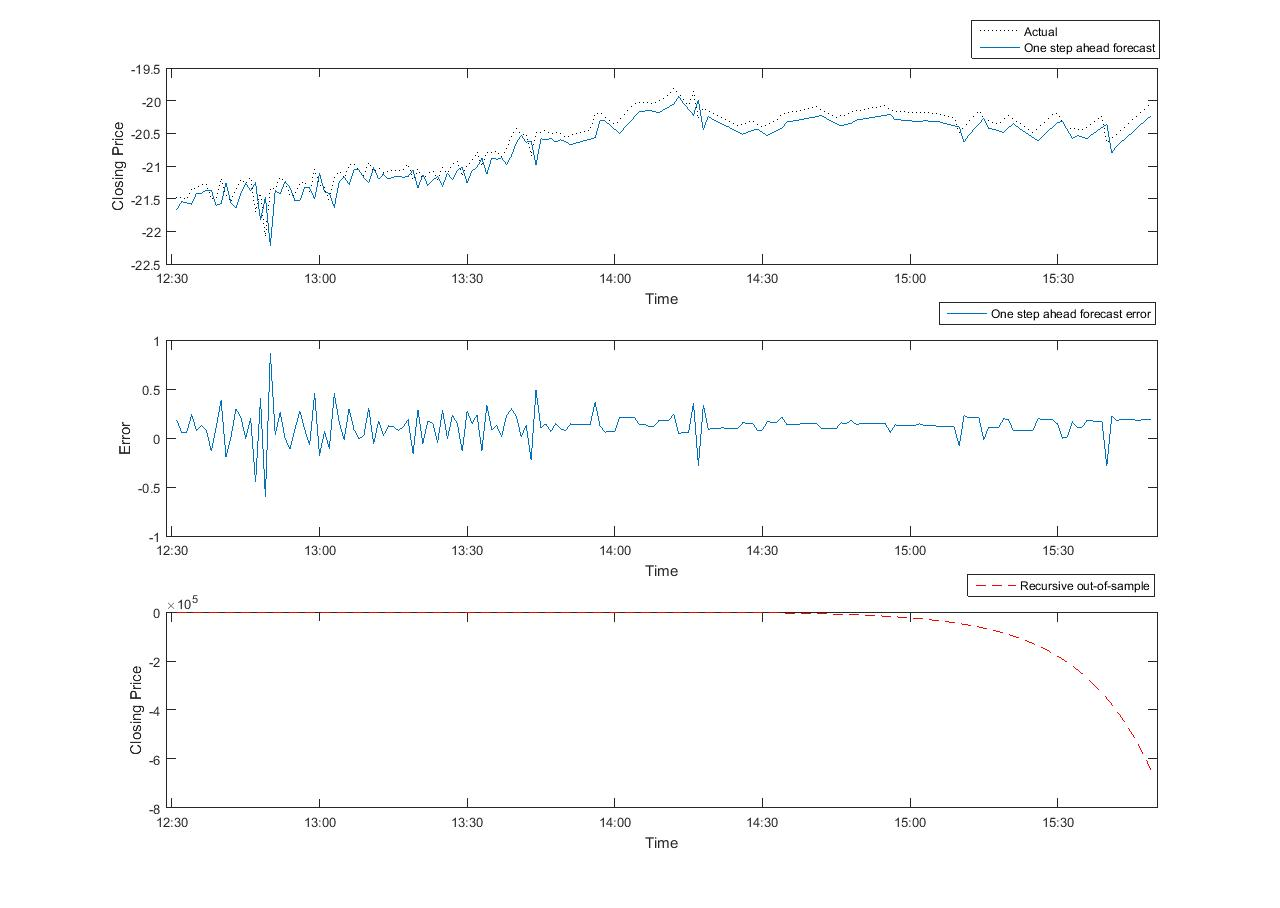
\includegraphics[width=\textwidth]{22linear}
\caption{Top: Time plot of linear model \ref{Equation 5.22} one-step forecast vs. actual values for the 22nd of September. Middle: Error value for each time point. Bottom: Time plot of recursive out-of-sample forecast using model \ref{Equation 5.22}}
\end{figure}

\paragraph{Sine function equations}\hfill \break
summary ...
\begin{equation}
\begin{align*}
close_{t} = 1.0728 * close_{t-10} + -0.359841 * close_{t-2} * sin ( -0.135171 * close_{t-10} + 3.33777 ) + -0.122294 \\ * close_{t-1} * sin ( -0.394844 * close_{t-1} + -6.05951
\end{align*}
\label{Equation 5.23}
\end{equation}

\begin{equation}
\begin{align*}
close_{t} = -1.00109 * close_{t-1} * sin ( -0.0343101 * close_{t-6} + 3.94084 ) + -0.081969 * sin ( 10 * close_{t-1} + -2.72036 )
\end{align*}
\label{Equation 5.24}
\end{equation}

\begin{table}[H]
\centering
\begin{tabular}{|l|l|l|l|}
\hline
\textbf{Dataset}                   & \textbf{Measure} & \textbf{\begin{tabular}[c]{@{}l@{}}Best Equation for \\ Training Set (Equation 5.23)\end{tabular}} & \textbf{\begin{tabular}[c]{@{}l@{}}Best Equation for\\ Test Set (Equation 5.24)\end{tabular}} \\ \hline
\multirow{4}{*}{\textit{Test set}} & MSE              & 0.3380121                                                                                          & 0.0230119                                                                                     \\ \cline{2-4} 
                                   & RMSE             & 0.5813881                                                                                          & 0.1516968                                                                                     \\ \cline{2-4} 
                                   & MFE              & 0.5290762                                                                                          & -0.0013418                                                                                    \\ \cline{2-4} 
                                   & MAD              & 0.5367762                                                                                          & 0.0999731                                                                                     \\ \hline
\textit{Training set}              & MSE              & 0.0587481                                                                                          & 0.0593866                                                                                     \\ \hline
\end{tabular}
\caption{Sine function results summary of best equations for the 22nd of September, 2015}
\label{nonlinear22tab}
\end{table}

\begin{figure}[H]
\centering
\label{VWNonlinear22fig}
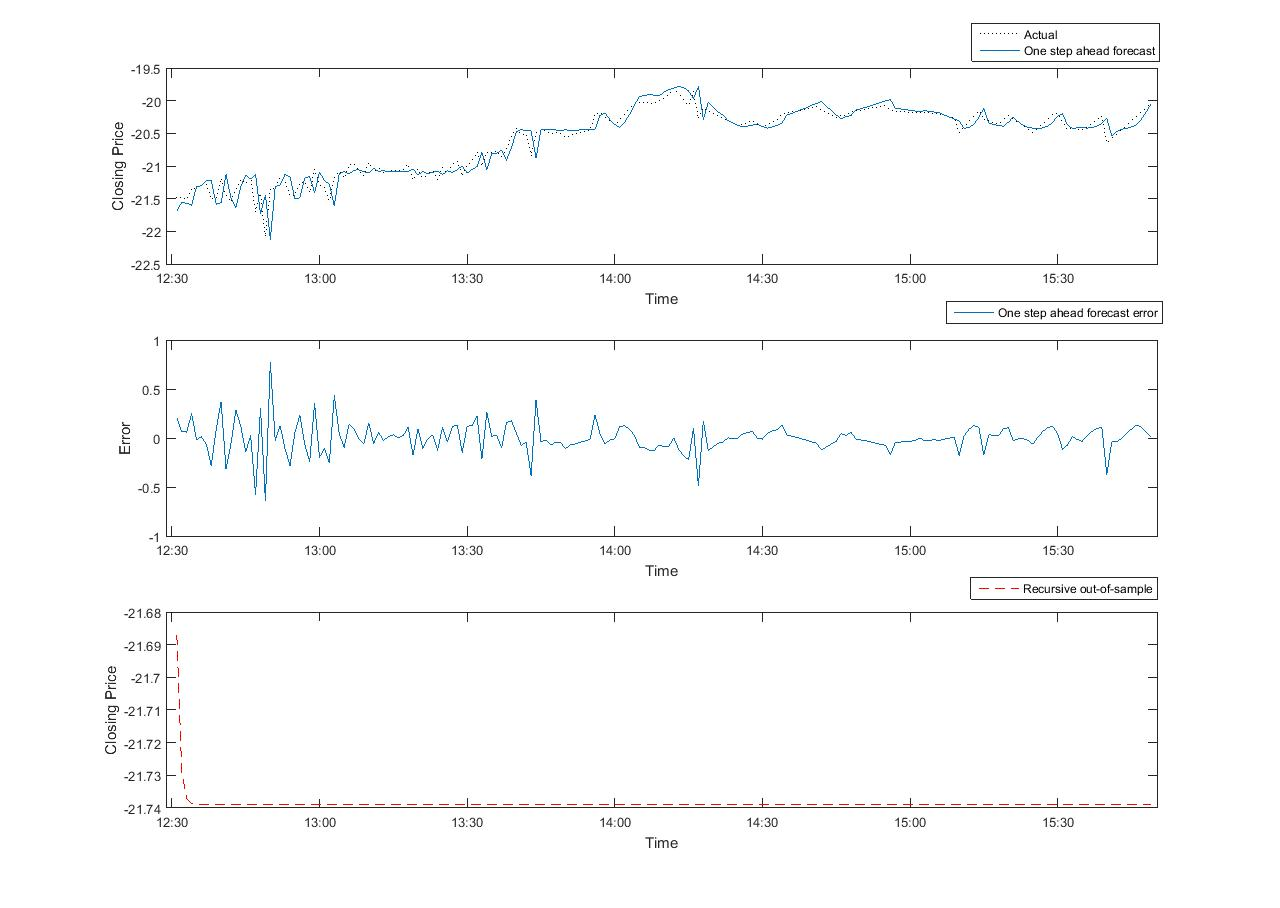
\includegraphics[width=\textwidth]{22nonlinear}
\caption{Top: Time plot of sine function model \ref{Equation 5.24} one-step forecast vs. actual values for the 22nd of September. Middle: Error value for each time point. Bottom: Time plot of recursive out-of-sample forecast using model \ref{Equation 5.24}}
\end{figure}

\subsection{23rd of September 2015}
\paragraph{Linear equations}\hfill \break
summary ...
\begin{equation}
\begin{align*}
close_{t} = -0.473019 + -0.163476 * close_{t-10} + 0.167391 * close_{t-9} + 0.949207 * close_{t-1} 
\end{align*}
\label{Equation 5.25}
\end{equation}
\begin{equation}
\begin{align*}
close_{t} = -0.41797 + -0.10875 * close_{t-5} + 0.0855231 * close_{t-7} + 0.981865 * close_{t-1}
\end{align*}
\label{Equation 5.26}
\end{equation}

\begin{table}[H]
\centering
\begin{tabular}{|l|l|l|l|}
\hline
\textbf{Dataset}                   & \textbf{Measure} & \textbf{\begin{tabular}[c]{@{}l@{}}Best Equation for \\ Training Set (Equation 5.25)\end{tabular}} & \textbf{\begin{tabular}[c]{@{}l@{}}Best Equation for\\ Test Set (Equation 5.26)\end{tabular}} \\ \hline
\multirow{4}{*}{\textit{Test set}} & MSE              & 0.0487654                                                                                          & 0.0428645                                                                                     \\ \cline{2-4} 
                                   & RMSE             & 0.2208288                                                                                          & 0.2070375                                                                                     \\ \cline{2-4} 
                                   & MFE              & 0.1809952                                                                                          & 0.1631283                                                                                     \\ \cline{2-4} 
                                   & MAD              & 0.1963118                                                                                          & 0.1831059                                                                                     \\ \hline
\textit{Training set}              & MSE              & 0.162616                                                                                           & 0.164765                                                                                      \\ \hline
\end{tabular}
\caption{Linear function results summary of best equations for the 23rd of September, 2015}
\label{linear23tab}
\end{table}

\begin{figure}[H]
\centering
\label{VWlinear23fig}
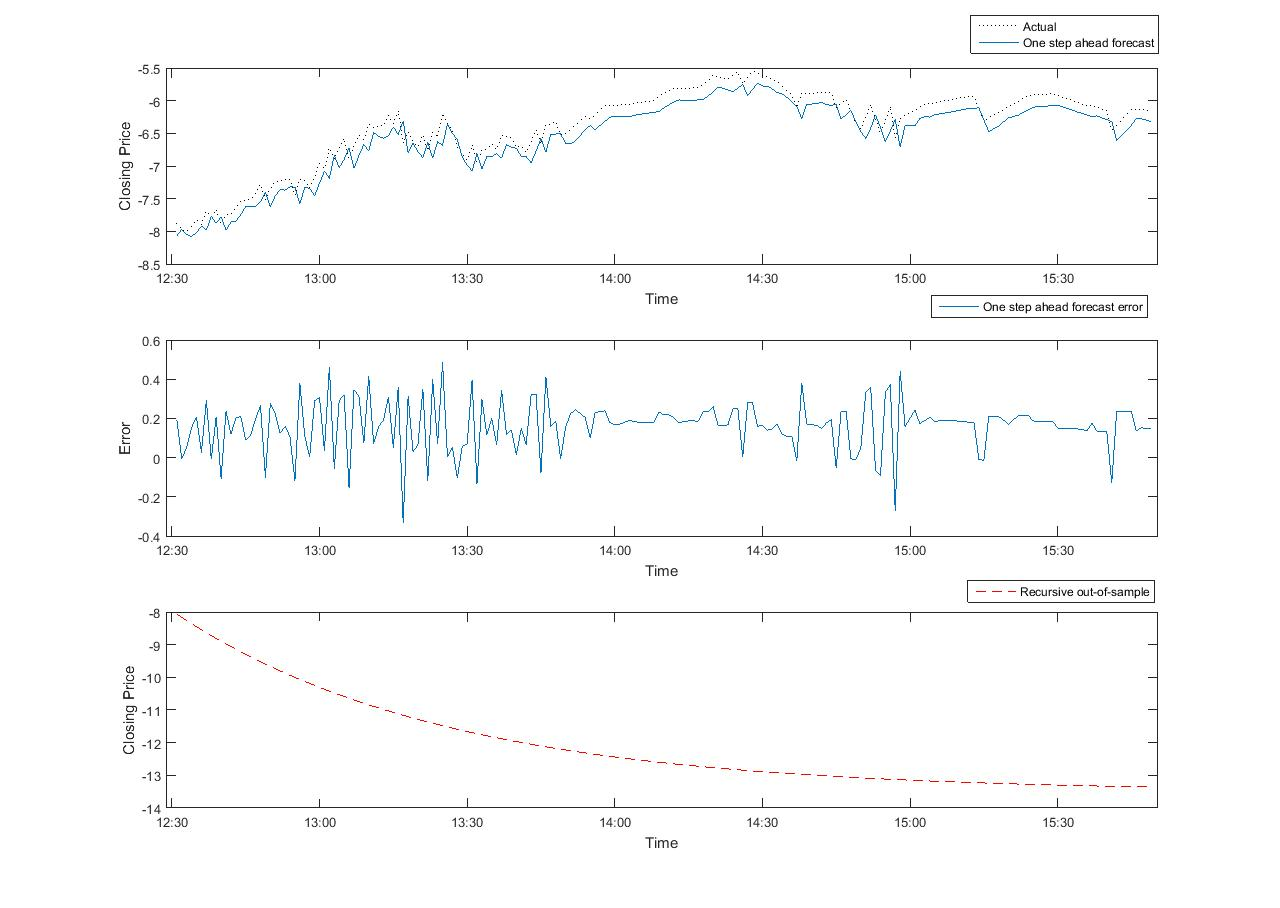
\includegraphics[width= \textwidth]{23linear}
\caption{Top: Time plot of linear model \ref{Equation 5.26} one-step forecast vs. actual values for the 23rd of September. Middle: Error value for each time point. Bottom: Time plot of recursive out-of-sample forecast using model \ref{Equation 5.26}}
\end{figure}

\paragraph{Sine function equations}\hfill \break
summary ...
\begin{equation}
\begin{align*}
close_{t} = -2.24703 + 0.796716 * close_{t-7} + 0.333022 * close_{t-10} * sin ( 0.232496 * close_{t-7} \\ + 2.27866 ) + 0.252547 * close_{t-1} * sin ( -0.412644 * close_{t-1} + -4.15913 )
\end{align*}
\label{Equation 5.27}
\end{equation}
\begin{equation}
\begin{align*}
close_{t} = 1.02448 * close_{t-7} + 0.248376 * close_{t-1} * sin ( -0.42099 * close_{t-1} + -4.25182 ) \\ + 0.401222 * close_{t-10} * sin ( 0.24787 * close_{t-7} + 2.44297 )
\end{align*}
\label{Equation 5.28}
\end{equation}

\begin{table}[H]
\centering
\begin{tabular}{|l|l|l|l|}
\hline
\textbf{Dataset}                   & \textbf{Measure} & \textbf{\begin{tabular}[c]{@{}l@{}}Best Equation for \\ Training Set (Equation 5.27)\end{tabular}} & \textbf{\begin{tabular}[c]{@{}l@{}}Best Equation for\\ Test Set (Equation 5.28)\end{tabular}} \\ \hline
\multirow{4}{*}{\textit{Test set}} & MSE              & 0.9387599                                                                                          & 0.4019836                                                                                     \\ \cline{2-4} 
                                   & RMSE             & 0.9688962                                                                                          & 0.6340218                                                                                     \\ \cline{2-4} 
                                   & MFE              & 0.9141880                                                                                          & 0.5744072                                                                                     \\ \cline{2-4} 
                                   & MAD              & 0.9141880                                                                                          & 0.5755946                                                                                     \\ \hline
\textit{Training set}              & MSE              & 0.143457                                                                                           & 0.144359                                                                                      \\ \hline
\end{tabular}
\caption{Sine function results summary of best equations for the 23rd of September, 2015}
\label{nonlinear23tab}
\end{table}

\begin{figure}[H]
\centering
\label{VWNonlinear23fig}
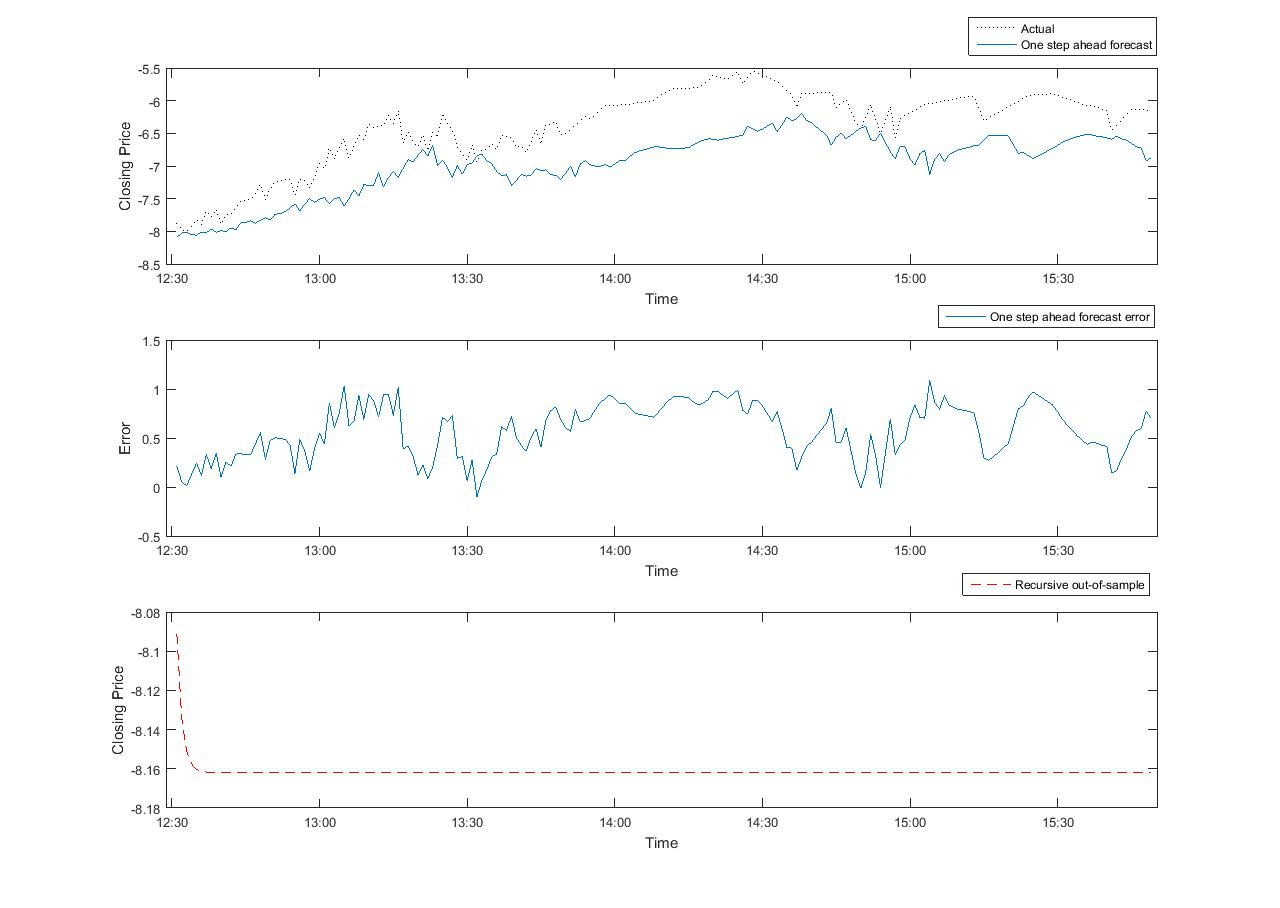
\includegraphics[width=\textwidth]{23nonlinear}
\caption{Top: Time plot of sine function model \ref{Equation 5.28} one-step forecast vs. actual values for the 23rd of September. Middle: Error value for each time point. Bottom: Time plot of recursive out-of-sample forecast using model \ref{Equation 5.28}}
\end{figure}

\section{Analysis of Methodology}
This chapter first evaluates the performance of the tools developed for the project
\chapter{Closing Remarks}
\section{Conclusion}
Applications and summary
\section{Further Work}

improvements: automate model generation from  Lagramge



\bibliography{bibilo}{}
\bibliographystyle{plain}
\end{document}   